\chapter{Second Chapter}
\section{Lattice Vibrations}
Lattice is defined as the periodic arrangement of atoms connected through elastic springs.\\
at $T=0\text{K}$, the energy of lattice is minimum and it will execute Simple Harmonic Motion(SHM)\\
at $T\neq0\text{K}$: as temparature increases particles start vibration and lattice energy increases oscillations will become anharmonic\\\\
\textbf{Vibration of 1-Dimensional monoatomic lattice}:
\begin{itemize}
	\item Number of atoms in primitive unit cell, P=1
\item Only nearest neighbours interaction is considered.
\item All atoms perform Simple Harmonic Motion 
\item $\omega^{2}=\frac{2 c}{m}(1-\cos k a)=\frac{4 c}{m} \sin ^{2}\left(\frac{k a}{2}\right)(\text{Dispersion Relation})$
\item Energy quanta of lattice vibration (elastic waves) is phonon.
\end{itemize}
\textbf{If $K$ is small ($\lambda$ large):}
\begin{align*}
k \rightarrow 0 &\quad \sin \left(\frac{k a}{2}\right) \simeq \frac{k a}{2}\\
\omega&=\sqrt{\frac{c}{m}} k a \Rightarrow \omega \propto k\\
Group velocity,V_{g}&=\frac{d \omega}{d k}=\sqrt{\frac{c}{m}} a\\
Phase velocity,V_{p}&=\frac{\omega}{k}=\sqrt{\frac{c}{m}} a\\
V g&=V_{P} \ \text { and independent of wave vector}, K
\end{align*}
 and at this wavelength, this medium behaves as non-dispersive medium\\
\textbf{If $K$ is large ($\lambda\rightarrow$ small)}:
\begin{align*}
\text { at the Brillouin zone boundary, } v_{g}&=0\\
v_{g}&=\frac{d \omega}{d k}=\sqrt{\frac{c}{m}} a\left|\cos \left(\frac{k a}{2}\right)\right|=0\\
\cos \frac{k a}{2}&=\cos \frac{\pi}{2}\\
\Rightarrow K&=\pm \pi / a \rightarrow \text { Boundary of Brillouin zone } \\
V_{p} &\neq V_{g} \text { hence it is, Dispersive medium. }\\
\omega_{\max }&=\sqrt{\frac{4 c}{m}} \sin ^{2}\left(\frac{k a}{2}\right)=\sqrt{\frac{4 c}{m}}
\end{align*}
\begin{figure}[H]
	\centering
	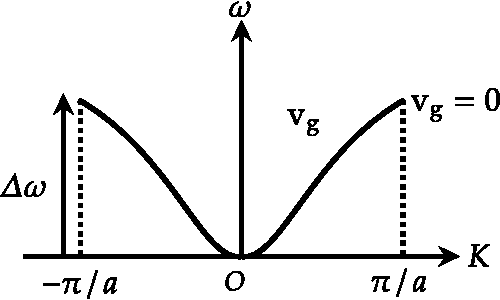
\includegraphics[height=3.3cm,width=4.8cm]{CP-1}
\end{figure}
\begin{align*}
\text { each Brillouin zone  }&\text{represents a Band, so band width}\\
\Delta \omega &=\omega_{\text {top }}-\omega_{\text {bottom }} \\
&=\sqrt{\frac{4 c}{m}}-0 \Rightarrow \sqrt{\frac{4 c}{m}}
\end{align*}
\subsection{Lattice Vibrations in 1-D diatomic lattice:}
$\text{Dispersion Relation}:$\\
$\omega_{\pm}^{2}=c\left(\frac{1}{m_{1}}+\frac{1}{m_{2}}\right) \pm c \sqrt{\left(\frac{1}{m_{1}}+\frac{1}{m_{2}}\right)^{2}-\frac{4 \sin ^{2}\left(\frac{k a}{2}\right)}{m_{1} m_{2}}}$\\
\textbf{(a) Optical Mode}\\
Optical Branch:
\begin{align*}
i)\quad \text { at }& K \rightarrow 0(\lambda \rightarrow \text { long }):\qquad\left(m_{1}<m_{2}\right)\\
&\sin \left(\frac{k a}{2}\right) \simeq 0\\
\omega_{+}^{2}&=2 c\left(\frac{1}{m_{1}}+\frac{1}{m_{2}}\right) \Rightarrow \omega_{+}=\sqrt{2 c\left(\frac{1}{m_{1}}+\frac{1}{m_{2}}\right)}
\end{align*}
\begin{align*}
ii)\quad \text { at } K=\pi/a \quad(\lambda \rightarrow \text { Short })\\
\sin \left(\frac{k a}{2}\right) &\approx 1 \Rightarrow \omega_{+}=\sqrt{\frac{2 c}{m_{1}}}
\end{align*}
\begin{itemize}
	\item At zone boundary $(K=\pm \pi/a)$, frequency of optical branch depends upon lighter mass.\item
Near centre of $BZ(K\approx 0)$, frequency of optical branch depends upon both masses.
\end{itemize}
\textbf{(b) Acoustical Branch}
\begin{align*}
\omega_{-}^{2}&=c\left(\frac{1}{m_{1}}+\frac{1}{m_{2}}\right)-c \sqrt{\left(\frac{1}{m_{1}}+\frac{1}{m_{2}}\right)^{2}-\frac{4 \sin ^{2}(k a / 2)}{m_{1} m_{2}}}\\
\text { i) at } k=0 \text { (centre of Brillouin zone}  \text { ): }&\\
\omega_{-}&=0 \quad \text{,Frequency of acoustical branch will be zero}\\
\text { ii) at } k \rightarrow 0 \text { (long wave length): }&\\
\sin ^{2}\left(\frac{k a}{2}\right) &\simeq \frac{k^{2} a^{2}}{4} \Rightarrow \omega_{-}=\sqrt{\frac{c}{2\left(m_{1}+m_{2}\right)}} k a\\
v_{g}&=\frac{d\omega}{d k}=\sqrt{\frac{c}{2\left(m_{1}+m_{2}\right)}} a\\
\text{iii) at Boundary }(k \rightarrow \pi / a):&\\
\omega_{-}^{2}&=\frac{2 c}{m_{2}} \Rightarrow \omega_{-}=\sqrt{\frac{2 c}{m_{2}}}
\end{align*}
\begin{figure}[H]
	\centering
	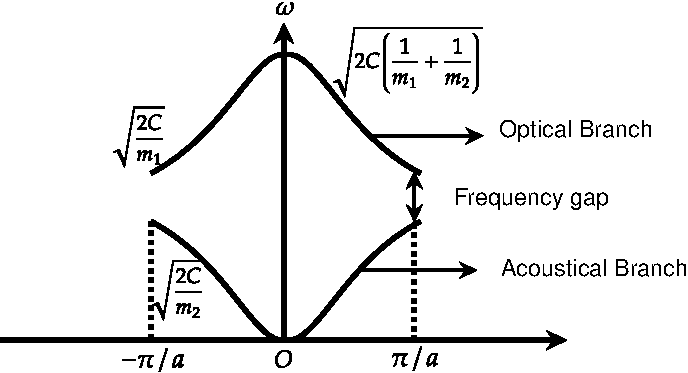
\includegraphics[height=4cm,width=7.5cm]{CP-2}
\end{figure}
\begin{itemize}
	\item Frequency gap $=\sqrt{\frac{2 c}{m_{1}}}-\sqrt{\frac{2 c}{m_{2}}} \Rightarrow \alpha\left(\sqrt{\frac{m_{2}}{m_{1}}}\right)^{2}$
	\item optical Branch: electro magnetic wave propagates in solid.\\ Acoustical: sound wave propagates in solid.
	\item Band width ($\Delta$w)\\
	for optical is
$	\sqrt{2 c}\left(\frac{1}{m_{1}}+\frac{1}{m_{2}}\right)-\sqrt{\frac{2 c}{m_{1}}}$
	  and for acoustical :$\sqrt{\frac{2 c}{m_{2}}} $
\end{itemize}
\renewcommand*{\arraystretch}{1.5}
\begin{tabular}{|c|c|c|c|} 
	\hline
	& $1Dimensional$ & $2Dimensional$ & $3Dimensional$ \\
	\cline { 2 - 4 } no. of Branches & $p$ & $2 p$ & $3 p$ \\
	\hline acoustical & 1 & 2 & 3 \\
	\hline optical & $p-1$ & $p-2$ & $p-3$\\
	\hline
\end{tabular}
\section{Thermal Properties of Solids}
\textbf{Classical Theory}(Dulong-Peptits theory)
\begin{itemize}
	\item Each atom is considered as 3-Dimensional Harmonic oscillator
	\item Internal Energy, $U=3NK_BT=3RT$
	\item $C_{V}=\frac{\partial U}{\partial T}=3 R$ (constant)
	\item  Valid for high temperature 
	\item  Fails at low temperature 
\end{itemize}
\textbf{Quantum theory}\\
Each atom is considered as Quantum Harmonic Oscillator
\begin{align*}
a)\quad \text{Einstein's Theory}:\\
C_V&=3R\left(\frac{\theta E}{T} \right) ^2 \frac{e^{\theta_{E/T}}}{(e^{\theta_{E/T}}-1)^2}\\
\text { at high temparature, } &C_{v} \approx 3 R \text { (valid) }\\
\text { at low temparature, }& C_{V}=3 R\left(\frac{\theta_{E}}{T}\right)^{2} e^{-\theta_{E} / T}\text { (invalid) }
\end{align*}
$b$)\quad \text{Debye Theory}:
\begin{itemize}
	\item Oscillators are now coupled and frequency of vibration depends on density of modes.
	\item $C_{V}$   at low temparature
	=$\frac{12}{5} \pi^{2} R\left(\frac{T}{\theta_{D}}\right)^{3}$ and
	$\theta_{D}=\frac{\hbar \omega_{D}}{K_{B}}$ (Debye temparature), Hence $C_{V}$ $\propto$ $T^{3}$ and it is valid with the experimentaly observed results 
	\item $C_{V}$   at High temparature $=3 R$ (valid) 
\end{itemize}
\section{ The classical Free Electron Theory of Metals (Drude-Lorentz Theory of Metals)} 
Drude and Lorentz proposed this theory in 1900. According to this theory, the metals containing the free electrons obey the laws of classical mechanics.
\subsubsection{Assumptions (salient features) in classical free electron theory}
	The classical free electron theory is based on the following postulates.
\begin{enumerate}
	\item  The valence electrons of atoms are free to move about the whole volume of the metal, like the molecules of a perfect gas in a container.
	\item The free electrons move in random direction and collide with either positive ions fixed to the lattice or the other free electrons. All the collisions are elastic in nature i.e., there is no loss of energy.
	\item The momentum of free electrons obeys the laws of the classical kinetic theory of gases.
	\item The electron velocities in a metal obey classical Maxwell-Boltzman distribution of velocities.
	\item When the electric field is applied to the metal, the free electrons are accelerated in the direction opposite to the direction of applied electric field.
	\item  The mutual repulsion among the electrons is ignored, so that they move in all the directions with all possible velocities.
	\item  In the absence of the field, the energy associated with an electron at temperature $T$ is given by $\frac{3}{2} k T$. It is related to the kinetic energy equation $\frac{3}{2} k T=\frac{1}{2} m v_{t h}^{2}$. Here $v_{t h}$ represents the thermal velocity.
\end{enumerate}
\subsection{Classical free electron theory-electrical conductivity}
The classical free electron theory was proposed by Drude and Lorentz. According to this theory the electrons are moving freely and randomly moving in the entire volume of the metal like gas atoms in the gas container. When an electric field is applied the free electrons gets accelerated. When an electric field $E$ is applied between the two ends of a metal of area of cross section A 
\begin{align*}
\text{Force acting on the electron in the electric field }&=e E\\
\text { From Newton's second law } F&=m a\\
\text { The acceleration of electron } a&=\frac{F}{m}=\frac{e E}{m}
\intertext{The average velocity acquired (i.e. drift velocity) by the electrons by the application of electric field is}
v_{d}&=a \tau=\frac{e E \tau}{m} \\
v_{d}&=a \tau=\frac{e E \tau}{m}=\frac{e E}{m} \frac{\lambda}{v_{r}}\\
\text { Where } v_{r}&=\text { RMS velocity. }\\
\text { The relation between current and drift velocity is }&\\
i&=n e A v_{d} \\
\text{The current density is }\quad j&=n e v_{d} \\
\text{Substituting the value of $\nu_d$ we get}\quad j&=\frac{n e^{2} E \tau}{m}\\
\text{Conductivity $\sigma$}\quad \sigma&=\frac{j}{E}=\frac{n e^{2} \tau}{m}\\
\text{Resistivity $\rho$}\quad\rho&=\frac{1}{\sigma}=\frac{m}{n e^{2} \tau} \\
\text{Mobility $\mu$}\quad \mu&=\frac{v_{d}}{E}=\frac{e \tau}{m}
\end{align*}
\subsection{Success of classical free electron theory}
1. It verifies ohm's law
2. It explains electrical conductivity of metals.
3. It explains thermal conductivity of metals.
4. It derives Widemann - Franz law. (i.e. the relation between electrical and thermal conductivity.
\begin{enumerate}
	\item It verifies ohm's law
	\item It explains electrical conductivity of metals.
	\item It explains thermal conductivity of metals.
	\item It derives Widemann - Franz law. (i.e. the relation between electrical and thermal conductivity.
\end{enumerate}
\subsection{Draw backs of classical free electron theory.}
\begin{enumerate}
	\item  It could not explain the photoelectric effect, Compton Effect and black body radiation.
	\item Electrical conductivity of semiconductors and insulators could not be explained.
	\item  Widemann - Franz law $\left(\frac{K}{\sigma T}=\right.$ constant $)$ is not applicable at lower temperatures
	\item Ferromagnetism could not be explained by this theory. The theoretical value of paramagnetic susceptibility is greater than the experimental value.
	\item According to classical free electron theory the specific heat of metals is given by $4.5 R$, where as the experimental value is given by $3 R$
	\item According to classical free electron the electronic specific heat is equal to $\frac{3}{2} R$ while the actual value is $0.01 R$
\end{enumerate}
\subsection{Sommerfeld's Quantum Theory for Electronic Heat Capacity}
Up to this point, we have only considered contributions to the heat capacity from vibrations within the solid. In metals, the free conduction electrons also contribute to the heat capacity. In the free electron model of metals, the conduction electrons are treated as a perfect gas obeying Fermi-Dirac statistic. Interactions of the electrons with the positively charged atomic ions and with the other electrons are neglected. This is not such a bad approximation as it may appear at first: the ions provide a positively charged background that partly screens the electrons from each other; and the residual collisions are often relatively unimportant - the energetically accessible final states are often already occupied, making any collisional excitation process forbidden by the Pauli exclusion principle. The first step in deriving the heat capacity is to determine the density of states. We will first do this in momentum space, and then transform the result into an expression describing the density of states per unit energy.
\subsubsection{Free electron gas in one dimensional box:}
We consider first a free electron gas in one dimension. We assume that an electron of mass $m$ is confined to a length $L$ by infinite potential barriers.
\begin{figure}[H]
	\centering
	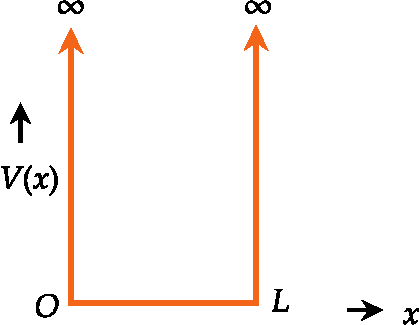
\includegraphics[height=3cm,width=4cm]{CMP-1}
\end{figure}
\begin{align*}
\mathrm{V}(\mathrm{x})=& 0 \text { for } 0<\mathrm{x}<\mathrm{L} \\
=& \infty \text { for } \mathrm{x} \leq 0 \text { and } \mathrm{x} \geq \mathrm{L}
\intertext{The wave-function $\psi_{n}$ of the electron occupying the $n^{\text {th }}$ state is determined from the solution of the Schrodinger equation i.e.}
\frac{d^{2} \psi_{n}}{d x^{2}}+\frac{2 m}{\hbar^{2}}\left(E_{n}-V\right) \psi_{n}&=0 \Rightarrow \frac{d^{2} \psi_{n}}{d x^{2}}+\frac{2 m}{\hbar^{2}} E_{n} \psi_{n}=0
\intertext{Note that this is a one-electron equation, which means that we neglect the electron-electron interactions. We use the term orbital to describe the solution of this equation.}
\text { The general solution to this equation is }&\\
\psi_{n}(x)&=A \sin K x+B \cos K x \quad \text { where } K=\sqrt{\frac{2 E m}{\hbar^{2}}}\\
\text { Boundary condition } \psi_{n}(0)&=0 \text { and } \psi_{n}(L)=0 \text { i.e. finally }\\
\text { Wave-function is } \psi_{n}(x)&=A \sin \left(\frac{n \pi}{L} x\right) \text {; }
\intertext{where $A$ is a constant and $n$ is an integer. From here, we obtain for the eigenvalues}
E_{n}&=\frac{n^{2} \hbar^{2} \pi^{2}}{8 m L^{2}} \text { where } A=\sqrt{\frac{2}{L}}
\end{align*}
These solutions correspond to standing waves with a different number of nodes within the potential well. Now we need to accommodate $N$ valence electrons in these quantum states. According to the Pauli exclusion principle no two electrons can have their quantum number identical. That is, each electronic quantum state can be occupied by at most one electron. The electronic state in a 1D solid is characterized by two quantum numbers that are $n$ and $m_{s}$, where $n$ describes the orbital $\psi_{n}(x)$, and $m_{s}$ describes the projection of the spin momentum on a quantization axis. Electron spin is equal to $\mathrm{S}=1 / 2$, so that there $(2 \mathrm{~S}+1)=2$ possible spin states with $m_{s}=\pm \frac{1}{2}$. Therefore, each orbital labelled by the quantum number $n$ can accommodate two electrons, one with spin up and one with spin down orientation.\\
Let $n_{F}$ denote the highest filled energy level, where we start filling the levels from the bottom $(n$ $=1$ ) and continue filling higher levels with electrons until all $N$ electrons are accommodated. It is convenient to suppose that $N$ is an even number. The condition $2 n_{F}=N$ determines $n_{F}$, the value of $n$ for the uppermost filled level. The energy of the highest occupied level is called the Fermi energy $E_{F}$, which will be solved in the next section. All the electronic levels are filled upto the Fermi energy. All the levels above are empty.
\subsubsection{Density of state}
 The Density of state is defined as no of electronic state present in a unit energy range, it is denoted by $\mathrm{D}(€)$ and is given by $D(\epsilon)=\left(\frac{d n}{d E}\right)$\\\\
Where $d n$ represents the no of electronic quantum states present in the energy interval $\mathrm{E}$ and $\mathrm{E}+$ $d E$, for a free electron gas, since each energy level contains two electronic states, one with spin up and the other with spin down. The value given by
\begin{align*}
D(\in)&=2\left(\frac{d n}{d E}\right) \Rightarrow \frac{d E}{d n}=\frac{\hbar^{2}}{2 m}\left(\frac{\pi}{L}\right)^{2} 2 n=\frac{h^{2} n}{4 m L^{2}} \Rightarrow D(\in)=2 \times\left(\frac{4 m L^{2}}{n h^{2}}\right)=\frac{8 m L^{2}}{h^{2}} \times \frac{L}{n}\\
\frac{1}{n}&=\left(\frac{h^{2}}{8 m L^{2} E}\right)^{1 / 2}\\
\text { Hence } D(E)&=\left(\frac{8 m L^{2}}{h^{2} E}\right)^{1 / 2}=\frac{4 L}{h}\left(\frac{m}{2 E}\right)^{1 / 2}
\end{align*}
\begin{figure}[H]
	\centering
	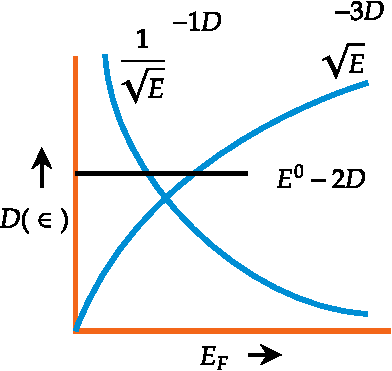
\includegraphics[height=3.5cm,width=3.5cm]{CMP-2}
\end{figure}
\begin{note}
	$\begin{array}{lr}D(E) \propto(E)^{-1 / 2} & \cdots \cdots 1 \mathrm{D} \\ \mathrm{D}(\mathrm{E}) \propto \mathrm{E}^{0} & \cdots2 \mathrm{D} \\ D(E) \propto \sqrt{E} & \cdots3 \mathrm{D}\end{array}$
\end{note}
\subsubsection{Filling of Energy level: Fermi-Dirac distribution function}
The Density of States tells us what states are available. We now wish to know the occupancy of these states. Electrons obey the Pauli exclusion principle. So, we may only have two electrons (one spin-up and one spin-down) in any quantum state. The distribution of electrons in the allowed energy level follows he Pauli's exclusion principle each energy level is doubly degenerate thus a total of $\mathrm{N}$ non-interacting electrons at ok can be filled in $\mathrm{N} / 2$ energy levels, the top most filled level is the $(\mathrm{N} / 2)$ th level and the level lying above it are empty. This level is therefore, the Fermi level as it divides the filled and empty levels at $0 \mathrm{k}$.\\
These electrons are rather distributed among the discrete energy level having energies ranging from 0 to $\mathrm{E}_{\mathrm{F} 0}$.
\begin{figure}[H]
	\centering
	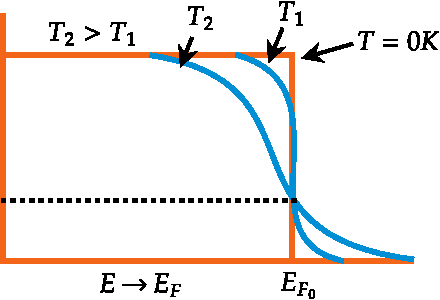
\includegraphics[height=3cm,width=4.5cm]{CMP-3}
\end{figure}
\begin{align*}
\text{The Fermi distribution function is }&\left.f(E)=\frac{1}{\left[e^{E-E_{F} / k T}+1\right.}\right]\text {for occupied }\text { At absolute zero the Equation }\\
\mathrm{F}(\mathrm{E})&=1 \quad \text { for } \quad \mathrm{E} \leq \mathrm{E}_{\mathrm{F} 0}\\
&=0 \quad \text { for } \quad \mathrm{E}>\mathrm{E}_{\mathrm{F} 0}
\intertext{The Fermi distribution function is a step function, at $0 \mathrm{~K}$. For temperature, greater than $0 \mathrm{~K}$ but less than the melting point of the metal such that $\mathrm{k}_{\mathrm{B}} \mathrm{T}<<\mathrm{E}_{\mathrm{F}}$ the distribution function loses its step character.}
\intertext{The probability of occupation $f(\mathrm{E})$ decreases gradually from 1 to 0 near EF this indicates that some of the state below $\mathrm{E}_{\mathrm{F}}$ are empty while some others above it are filled. This is because some of the electrons from the energy state below $\mathrm{E}_{\mathrm{F}}$ gain thermal energy and get excited to the state above $\mathrm{E}_{\mathrm{F}}$ at $\mathrm{E}=\mathrm{E}_{\mathrm{F}}$}\\
f\left(E_{F}\right)&=\frac{1}{2}
\end{align*}
\subsubsection{Density of State in Three Dimensions:}
\begin{figure}[H]
	\centering
	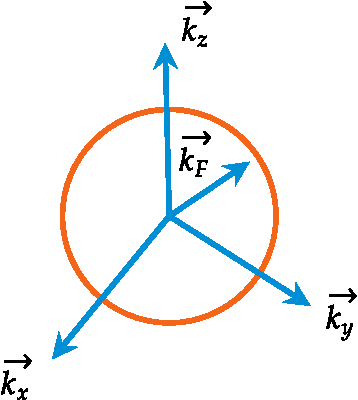
\includegraphics[height=3.3cm,width=3cm]{CMP-4}
\end{figure}
\begin{align*}
\text { Fermi energy is given as } E_{F}&=\frac{p^{2}}{2 m}=\frac{h^{2} K_{E}^{2}}{2 m}\\
E_{F}&=\frac{\hbar^{2}}{2 m} K_{F}^{2} \text { where } \mathrm{K}_{\mathrm{F}} \text { is Fermi radius } K_{F}=\left(\frac{3 \pi^{2} N}{V}\right)^{1 / 3}\\
E_{F}&=\frac{\hbar^{2}}{2 m}\left(\frac{3 \pi^{2} N}{V}\right)^{2 / 3}=E_{F}=3.65 \times 10^{-19} n^{2 / 3} \mathrm{eV}
\intertext{i.e. $\mathrm{E}_{\mathrm{F}}$ depends on both the Electronic concentration and mass}
	\text { The Total no. of electron is Therefore } N&=\frac{V}{3 \pi^{2}} K_{F}^{3}=\frac{V}{3 \pi^{2}}\left(\frac{2 m E_{F}}{\hbar^{2}}\right)^{3 / 2}
	\intertext{$\therefore$ Total No of state is equal to the total No of electron is i.e}
	\int_{0}^{E_{F}} D(E) d E&=N=\frac{V}{3 \pi^{2}}\left(\frac{2 m E_{F}}{\hbar^{2}}\right)^{3 / 2} \\
	\int D(\in) d E&=\int \frac{V}{2 \pi^{2}}\left(\frac{2 m}{\hbar^{2}}\right)^{3 / 2} E^{1 / 2} d E \\
	D(\in)&=\frac{V}{2 \pi^{2}}\left(\frac{2 m}{\hbar^{2}}\right)^{3 / 2} E^{1 / 2} \quad \Rightarrow \quad D(\in) \propto \sqrt{E}-3 D
	\intertext{This result may also be obtained and expressed in a simple way by taking the natural logarithm of expression}
	\ln N&=3 / 2 l_{n} E_{F}+\operatorname{cons} \tan t\\
	\frac{d N}{N}&=\frac{3}{2} \frac{d E_{F}}{E_{F}} \quad \text { or } \quad \frac{d N}{d E_{F}}=3 / 2\left(\frac{N}{E_{F}}\right) \quad \text { at } \quad E=E_{F}
	\intertext{The Density of filled electronic state $\mathrm{N}(E)$, at any temperature $T$ is obtain by multiplying the density of state $\mathrm{D}(\mathrm{E})$ at $0 \mathrm{~K}$ by probability occupation $f(\mathrm{E})$ of the quantum state $\mathrm{E}$ at that temperature.}
	N(\in)&=D(\in) f(E) \\
	N(\in) d E&=D(\in) f(E) d E
\end{align*}
\subsubsection{Fermi Energy $\left(\mathbf{E}_{\mathrm{F} 0}\right)$ }
 Fermi energy is an important parameter, which can be determined by the following method. If the total number of free electrons in a metal is $\mathrm{N}$, then we have
\begin{align*}
N&=\int_{0}^{\infty} N(\in) d E=\int_{0}^{\infty} D(\in) f(E) d E \\
&=\frac{V}{2 \pi^{2}}\left(\frac{2 m}{\hbar^{2}}\right)^{3 / 2} \int_{0}^{\infty} E^{1 / 2} f(E) d E \\
&=\frac{V}{2 \pi^{2}}\left(\frac{2 m}{\hbar^{2}}\right)^{3 / 2}\left[\int_{0}^{E_{F 0}} E^{1 / 2} f(E) d E+\int_{E_{F 0}}^{\infty} E^{1 / 2} f(E) d E\right] \\
&\varepsilon<E_{F} 1 \\
&=\frac{V}{2 \pi^{2}}\left(\frac{2 m}{\hbar^{2}}\right)^{3 / 2} \int_{0}^{E_{F 0}} E^{1 / 2} d E \\
&E_{F 0}=\frac{\hbar^{2}}{2 m}\left(\frac{3 \pi^{2} N}{V}\right)^{2 / 3}=\frac{\hbar^{2}}{2 m}\left(3 \pi^{2} n\right)^{2 / 3} \Rightarrow E_{F} \propto n^{2 / 3}\\
\text { Where } n&=\frac{N}{V} \text { is the number density of electrons (number of electrons per unit volume). }
\end{align*}
\subsubsection{Average Kinetic Energy $\bar{E}$}
\begin{align*}
\bar{E}_{0}&=\frac{1}{N} \int_{0}^{\infty} E D(E) f(E) d E \\
\bar{E}_{0}&=\frac{V}{2 \pi^{2}}\left(\frac{2 m}{\hbar^{2}}\right)^{3 / 2} \frac{1}{N}\left[\int_{0}^{E_{F_{0}}} E E^{1 / 2} f(E) d E+\int_{E_{F}}^{\infty} E E^{1 / 2} f(E) d E\right]\\
&=\frac{V}{2 \pi^{2}}\left(\frac{2 m}{\hbar^{2}}\right)^{3 / 2} \frac{1}{N} \int_{0}^{E_{F 0}} E^{3 / 2} d E=\frac{2}{5} \frac{V}{2 \pi^{2}}\left(\frac{2 m}{\hbar^{2}}\right)^{3 / 2} \frac{1}{N} E_{F}^{5 / 2} \\
\bar{E}_{0}&=\frac{3}{5} E_{F 0} \quad-\cdots 3 \mathrm{D}
\end{align*}
\begin{note}
	\begin{align*}
		&\text {  Average }\text{energy in 1-dimension and 2-dimensions are also written as }\\
&\left.\begin{array}{ll}
\bar{E}&=\frac{1}{3} E_{F}  ----1 D \\
\bar{E}&=\frac{1}{2} E_{F}  ----2 D
\end{array}\right\}
	\end{align*}
\end{note}
\subsubsection{Electron Specific heat:}
The Free electron gas model explains the electronic to specific heat of metals by restricting the No of electrons contributing to specific heat to $\mathrm{N}\left(\mathrm{K}_{\mathrm{B}} \mathrm{T} / \mathrm{E}_{\mathrm{F}}\right)$. It yielded the expression for specific heat as
$$C_{V}=\frac{3}{2} N K_{B}\left(\frac{K_{B} T}{E_{F}}\right) \Rightarrow C_{V} \approx \frac{3}{2} N K_{B}\left(\frac{T}{T_{F}}\right), \quad C_{V} \propto\left(\frac{T}{T_{F}}\right)$$
\section{Band Theory of Solid}
The failure of the free electron model is due to the over simplified assumption that a conduction electron in a metal experiences a constant or zero potential due to the ion cores and hence is free to move about crystal. Now the periodic potential described above forms the basis of the band Theory of solids. The behavior of an electron in this potential is describe by constructing the electron wave functions using One-electron approximates. As we shall discuss later, the motion of an electron in a periodic potential yields the following results.
\begin{enumerate}[label=\alph*)]
	\item There exists an allowed energy band separated by forbidden region or band gap.
	\item  The electronic energy function $\mathrm{E}(\mathrm{K})$ are periodic in the wave vector $\mathrm{K}$\\
	In the free electron Theory $\mathrm{E}$ varies with $\mathrm{K}$
	$$
	E_{K}=\frac{\hbar^{2} k^{2}}{2 m}
	$$
\end{enumerate}
\subsection{The Bloch Theorem}
Bloch's theorem is just a way to describe the wavefunction for periodic solids. Bloch's theorem constrains $\psi$ and thus $E$ for periodic solids.
The 1-D Schrödinger equation for an electron moving in a constant potential $V_{0}$ is $\frac{d^{2} \psi}{d x^{2}}+\frac{2 m}{\hbar^{2}}\left(E-V_{0}\right) \psi=0 . \quad$ The solution $\psi(\mathrm{x})=\mathrm{e}^{\pm i \mathrm{kx}}$
For periodic potential with period equal to the lattice constant a we have
$$
\psi(\mathrm{x})=\mathrm{e}^{\pm \mathrm{ikx}} \mathrm{U}_{\mathrm{k}}(\mathrm{x}) \quad \text { where } \mathrm{U}_{\mathrm{k}}=\mathrm{U}_{\mathrm{k}}(\mathrm{x}+\mathrm{a})
$$
Bloch's theorem in 3-dimensions: Bloch's theorem contains two postulates
\begin{enumerate}
	\item  Because we have a solid that is periodic at the atomic scale, we get a traveling wave solution $\left(e^{i \vec{k} \cdot \vec{r}}\right)$ for $\psi$ that is modulated by the translational symmetry of the lattice $\left(u_{\vec{k}}\right)$
	$$
	\psi_{k}(\vec{r})=u_{k}(\vec{r}) e^{i \vec{k} \cdot \vec{r}} \quad \text { where } \quad u_{k}(\vec{r})=u_{k}(\vec{r}+\vec{T})
	$$
	Here, wavefunction reflects the symmetry of the lattice via $u_{k}(\vec{r})$ and Traveling wave solution suggests that we must have invoked periodic boundary conditions for the macroscopic solid.
	\item Alternatively, we can describe the wavefunction a $\psi_{k}(\vec{r}+\vec{T})=c \psi_{k}(\vec{r})$. Which is to say, in a slightly different way, the wavefunction at $r+T$ is very related to the wavefunction at $\mathrm{r}$. Here, $\mathrm{c}$ is a modulation term, we'll explore in detail below
\end{enumerate}
\subsection{The Kronig-Penney Model}
This model illustrates the behavior of electrons in a periodic potential by assuming a relatively simple one-dimensional model of periodic potential as shown figure.\\
For this potential write down the Schrödinger wave equation and its general solution with taking potential constant finally. We get
$$
P \cdot \frac{\sin \alpha a}{\alpha a}+\cos \alpha a=\cos k a \quad \text { where } P=\frac{m V_{0} b a}{\hbar^{2}}
$$
which is a measure of the area $V_{0} b$ of the potential barrier. Thus, increasing $\mathrm{P}$ has the physical meaning of bonding an electron more strongly to a particular potential well
$$\frac{1}{\alpha a} \sin \alpha a+\cos \alpha a$$
$$\text { We know that } E=\frac{\alpha^{2} \hbar^{2}}{2 m}=\frac{\pi^{2} \hbar^{2}}{2 m a^{2}} n^{2}$$
It may be noted that since $\alpha^{2}$ is proportional to the energy $E$ the abscissa is a measure of the energy. The following conclusion may be drawn from figure.
\begin{enumerate}[label=\roman*)]
	\item The energy spectrum of the electrons consists of alternate regions of allowed energy bands (solid lines on abscissa) and forbidden energy band (broken lines)
	\item The width of the allowed energy bands increases with $\alpha a$ or the energy
	\item The width of particular allowed energy band decreases with increase in value of $P$.
\end{enumerate} 
Figure- Allowed (shaded) and forbidden (open) energy ranges as a function of $P$\\
Energy Verses Wave-Vector relationship\\
The energy $E$ is also an even periodic function of $k$ with period of $2 \pi / a$ i.e $k=\pm n \pi / a$
\begin{align*}
d n&=\frac{l}{2 \pi} d k\\
\text{Velocity is }v&=\frac{1}{\hbar} \frac{d E}{d k}.
\end{align*}
\subsection{Concept of effective mass electrons and Holes}
In one dimension, an electron with wave-vector $k$ has group velocity
\begin{align*}
v&=\frac{d \omega}{d k}=\frac{1}{\hbar} \frac{d E}{d k}\\
\text { If an electric field } \varepsilon &\text { acts on the electron, then in time } \delta t \text {. It will do work }\\
\delta E&=\text { force times distance }=-e \varepsilon v \delta t \\
\text{But}\quad \delta E&=\frac{d E}{d k} \delta k=\hbar v \delta t\\
\text { So, comparing equation  }&\text{(ii) with (iii), we have}\\
\delta k&=-\frac{e \varepsilon}{\hbar} \delta t, \quad \text { or } \quad \hbar \frac{d k}{d t}=-e \varepsilon\\
\text { In terms of force } F, \quad \hbar \frac{d k}{d t}&=F\\
\text { Generalising to three dimensions: } v&=\frac{1}{\hbar} \nabla_{k} E\\
\text { where } \nabla_{k}=\hat{i} \frac{d}{d k_{x}}+\hat{j} \frac{d}{d k_{y}}+\hat{k} \frac{d}{d k_{z}} \quad &\text { and } \quad \hbar \frac{d k}{d t}=F\\
\text{From equation }
(i) v&=\frac{d \omega}{d k}=\frac{1}{\hbar} \frac{d E}{d k},\\
\text { Differentiating with respect to time } \frac{d v}{d t}&=\frac{1}{\hbar} \frac{d^{2} E}{d k d t}=\frac{1}{\hbar} \frac{d^{2} E}{d k^{2}} \frac{d k}{d t}\\
\text { But from equation (iv), } \hbar \frac{d k}{d t}&=F\\
\text{So }
\frac{d v}{d t}&=\frac{1}{\hbar^{2}} \frac{d^{2} E}{d k^{2}} F\\
\text { But from Newton's equation we expect } \frac{d v}{d t}&=\frac{1}{m} F\\
\text{which leads us to define an effective mass }
\frac{1}{m^{*}}&=\frac{1}{\hbar^{2}} \frac{d^{2} E}{d k^{2}}
\end{align*}
That is\\
The dynamics of electrons is modified by the crystal potential;\\
The effective mass depends on the curvature of the bands;\\
Flat bands have large effective masses;\\
Near the bottom of a band, $m^{*}$ is positive, near the top of a band, $m^{*}$ is negative.\\
\subsubsection{Hole Concept}
\textbf{Hole wavevector:} The total $k$ of a full band is zero: if we remove an electron with wavevector $k_{e}$ the total $k$ of the band is $k_{h}+k_{e}=0 \Rightarrow k_{h}=-k_{e}$\\
\textbf{Hole energy:} Take the energy zero to be the top of the valence band. The lower the electron energy, the more energy it takes to remove it; thus
\begin{align*}
E_{h}\left(k_{h}\right)&=-E_{e}\left(k_{e}\right)\\
\text { But bands are usually symmetric, }& \quad E(k)=E(-k)\\
\text{So}\quad E_{h}\left(k_{h}\right)&=E_{h}\left(-k_{h}\right)=-E_{e}\left(k_{e}\right)
\end{align*}

\begin{align*}
\text{Hole velocity: In three dimensions}\\
v_{h}&=\frac{1}{h} \nabla_{k_{h}} E_{h}\\
\text{But}\quad k_{h}&=-k_{e} \quad\text{So}\quad \nabla_{k_{h}}=-\nabla_{k_{e}}\\
\text{and so}\quad v_{h}&=-\frac{1}{\hbar} \nabla_{k_{e}}\left(-E_{e}\right)=v_{e}
T\end{align*}
The group velocity of the hole is the same as that of the electron.\\
\textbf{Hole effective mass:} The curvature of $E$ is just the negative of the curvature of $-E$,
So
$$
m_{h}^{*}=-m_{e}^{*}
$$
Note that this has the pleasant effect that if the electron effective mass is negative, as it is at the top of the band, the equivalent hole has a positive effective mass.
\subsubsection{Hole dynamics}
\begin{align*}
\text{We know that}\quad \hbar \frac{d k_{e}}{d t}&=-e\left(\varepsilon+v_{e} \times B\right)\\
\text{Substituting}\quad k_{h}&=-k_{e} \text { and } v_{h}=v_{e} \text { gives }\\
\hbar \frac{d k_{h}}{d t}&=e\left(\varepsilon+v_{h} \times B\right)
\end{align*}
Exactly the equation of motion for a particle of positive charge.\\
Under an electric field, electrons and holes acquire drift velocities in opposite directions, but both give electric current in the direction of the field. 2. Radius of the Fermi sphere in $\mathrm{K}-$ space is given by


\section{Semiconductor}
$\left.\begin{array}{l}\mathrm{Eg}\left(s_{i}\right)=1.1 \mathrm{eV} \\ \mathrm{Eg}(\mathrm{he})=0.7 \mathrm{eV}\end{array}\right] \rightarrow$
elementry semiconductor\\
$Eg (haAs )=1.43 ev ]\rightarrow$ compound semiconductor.
\begin{itemize}
	\item Their conductivity can be modified according to application by changing doping concentration.
	\item Higher band gap means lower reverse saturation current, therfore thermal stability of $Si$ is better than $Ge$\\
	Pe ${Si}$ is better than $Ge$.
\end{itemize}
\subsubsection{According to Band Gap}
1.\quad \textbf{Direct Band gap semiconductor}
\begin{figure}[H]
	\centering
	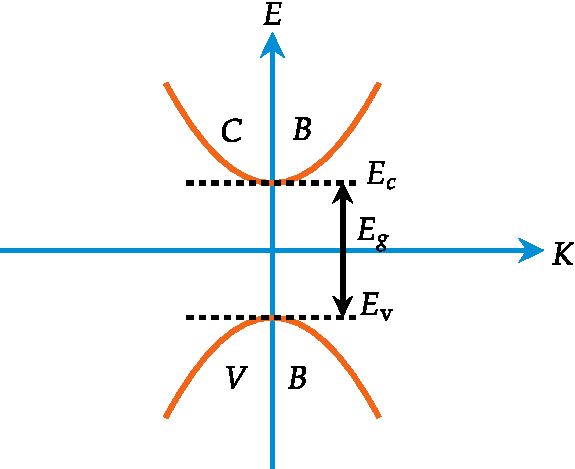
\includegraphics[height=3.5cm,width=4cm]{CMP-16}
	\caption{}
	\label{}
\end{figure}
$e^{\ominus}$ directly jump from top of V.B to bottom of C.B
\begin{itemize}
	\item No of energy or momentum of incident photon is transferred to the phonon.\\
	i.e no phonon involvement
	\item Semiconductor entire energy is absorbed or emitted in the form of optical energy.\\
	$\lambda=\frac{h c}{E g}$ (Used in light-emitting applications)
	\item example: cdsi, GaAs, Cds ete.
\end{itemize}
2.\quad \textbf{Indirect Band Gap Semiconductor}
\begin{figure}[H]
	\centering
	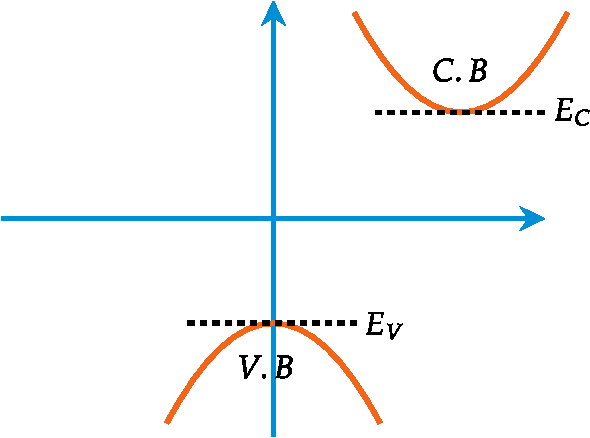
\includegraphics[height=3.5cm,width=4.5cm]{CMP-17}
	\caption{}
	\label{}
\end{figure}
\begin{itemize}
	\item Some energy or momentum of incident photon is transferred to the phonon, to jump $e^\ominus$ From top of $U \cdot B$ to Bottom of $C \cdot B$ i.e phonon involvement.
	\item Here, some part of energy is converted into heat. Hence, don't used for light emitting applications.
	\item examples: si, Ge, sic etc.
	According to Doping Concentration
	1.Intrinsic Semiconductor (Undoped/Pure)\\
	Behaves as insulator at $t=$0K
\end{itemize}
\begin{figure}[H]
	\centering
	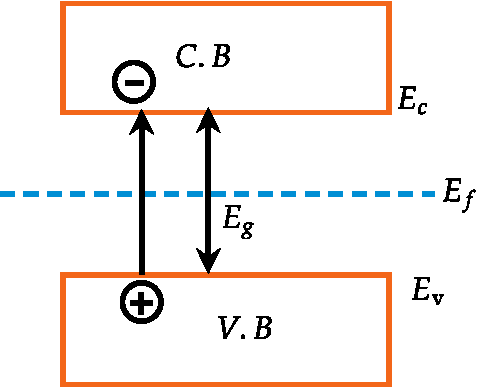
\includegraphics[height=3cm,width=3.8cm]{CMP-18}
	\caption{}
	\label{}
\end{figure}
\begin{align*}
E g&=E_{C}-E_{V}\\
E_{F}&=\frac{E_{C}-E_{v}}{2} \text { at } T=O K
\end{align*}
Hole: Vacancy of $e^{\ominus}$, it is a fermion.
\begin{align*}
e^{\ominus} \operatorname{conc} \cdot(n)=\frac{\text { no. of } e^{\ominus }\&}{\text { volume }}\\
\text { hole concentration }(p)&=\frac{\text { no.of holes }}{\text { vol. }}\\
n_{i}=D_{i}&=\left(N_{c} N_{U}\right)^{1 / 2} e^{-E g\left(2 k_{B} T\right.}\\
\text { intrinsic carrier conc. }&\\
N_{C}=2\left(\frac{2 \pi m e^{*} K_{B} t}{R^{2}}\right)^{3 / 2}\qquad& N_{V}=2\left(\frac{2 \pi m_{R}^{*} K_{B} T}{\hbar^{2}}\right)^{3 / 2}\\
\text { Dos at CB edge }\hspace{2cm}&\text { DOS at } V B \text { edge. }\\
n_{i}&=c T^{3 / 2} \exp \left(-\frac{E g}{2 K_{B} T}\right)\\
\ln n_{i}&=\ln (c)+\frac{3}{2} \ln T-\frac{E g}{2 k_{B} T}
\end{align*}
\begin{figure}[H]
	\centering
	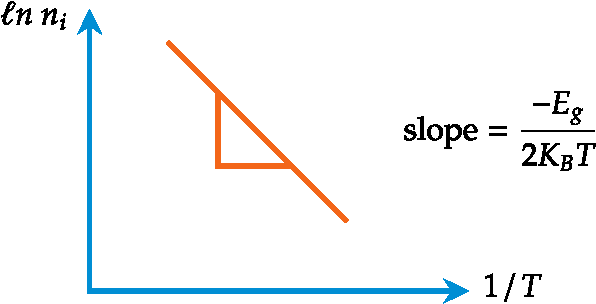
\includegraphics[height=3cm,width=5cm]{CMP-19}
	\caption{}
	\label{}
\end{figure}
conductivity:
\begin{align*}
\sigma&=n e H_{e}+p e H_{h}\\
\sigma&=n_{i} e\left(\mu_{e}+\mu_{h}\right)\\
\sigma_{i}&=\left[c T^{3 / 2} \exp \left(\frac{-E g}{2 K_{B} T}\right)\right]
\end{align*}
\begin{figure}[H]
	\centering
	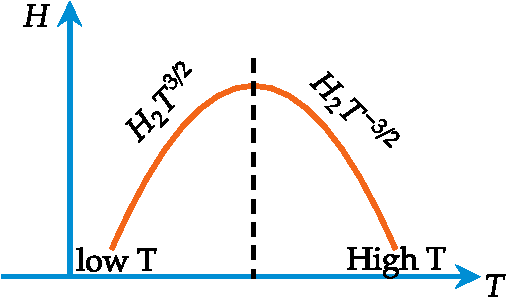
\includegraphics[height=3cm,width=5cm]{CP-4}
	\caption{}
	\label{}
\end{figure}
\begin{align*}
\text { exact position  }&\text{of fermi level at temp. T}\\
E_{F}&=\left(\frac{E_{C}+E_{v}}{2}\right)+\frac{3}{4} k_{B} T \ln \left(\frac{m_{R}^{*}}{m_{e}^{*}}\right)\\
\text { Position of  }&\text{fermi level Relative to V.B}
\end{align*}
\begin{figure}[H]
	\centering
	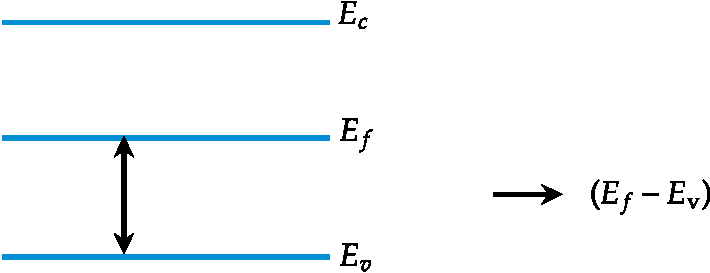
\includegraphics[height=2cm,width=5cm]{CMP-20}
	\caption{}
	\label{}
\end{figure}
\begin{align*}
\text { at } T&=0 K\\
E_{F}-E_{V}&=\left(\frac{E_{C}-E_{V}}{2}\right)+\frac{3}{4} K_{B} T \ln \left(\frac{m_{R}^{*}}{m_{e}^{*}}\right)
\end{align*}
2.\textbf{Extrinsic Semiconductor}\\
1. $n-$ type:
\begin{itemize}
	\item  electrons are majority charge carriers\\
	\item formed by doping the infrinsic si with pentavalent impurities like $P, A \&$, Sb, Bi etc
	\begin{figure}[H]
		\centering
		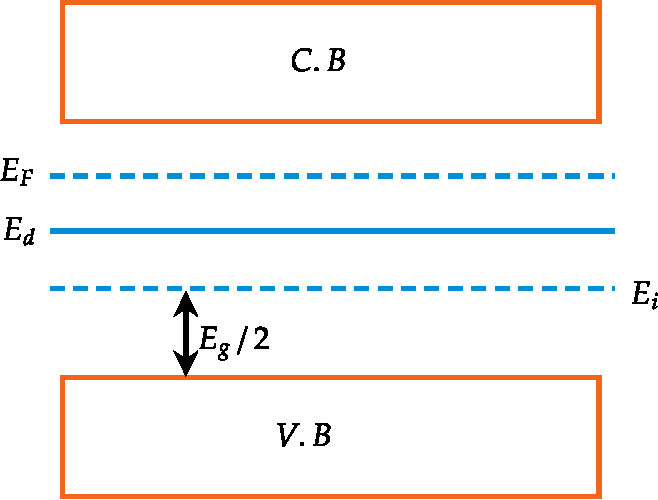
\includegraphics[height=3.5cm,width=4cm]{CMP-21}
		\caption{}
		\label{}
	\end{figure}
	at $T$ increases $E_F$ will moves towards $E_i$\\
	at $T=0K$
	\item $n$-type semiconductor is electrcally newral i.e net charge $=0$\\
	\item majority carier conc. $(n)=$ doner density $\left(N_{d}\right)$\\
	\item $K_{B T}=25 \mathrm{meV}$ at $T=300 \mathrm{~K}$\\
	\item as $T$ Tes, Ef will moves touards $E_{i}$\\
	\item $N_{d}$ remains constant at all temperatures\\
	\item extrinsic semiconductor will become intrinsic semiconductor by raising the temperature and by doping opposite type of impurity.
\end{itemize}
\textbf{Law of Mass Action}\\
By this law we can calculate majosity and minority carrier concentration.
\begin{align*}
\text { majority carrier conc. }(n)&=\text { donor conc. }\left(N_{d}\right)\\
\text { minority conc.}&= p\\
n p&=n i p_{i}\\
n p&=n i^{2}
\end{align*}
\textbf{Conductivity :}
\begin{align*}
\sigma&=n e \mu_{e}+p e \mu_{h} \\
\sigma &\approx n e \mu_{e}
\end{align*}
ii) p-type: 
\begin{itemize}
	\item holes are majority charge carriers 
	\item formed by doping the intrinsic si with\\
	fivalent impurity like $B, h a$, In, Al etc.
	\begin{figure}[H]
		\centering
		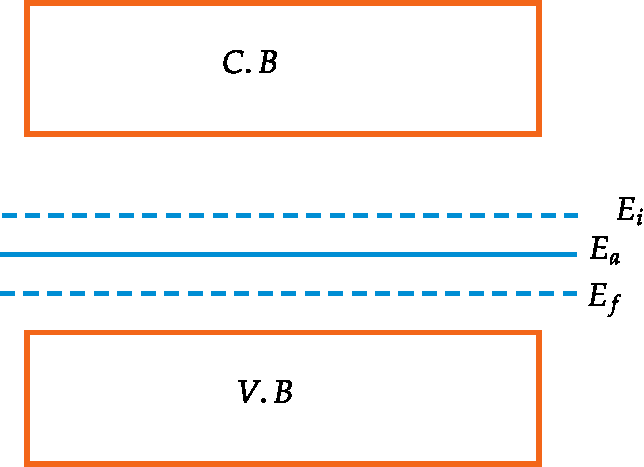
\includegraphics[height=3cm,width=5cm]{CMP-22}
		\caption{}
		\label{}
	\end{figure}
	as teperature increases $E_F$ will moves towards $E_i$\\
	i.e. extrinsic s/c becomes intrinsic semiconductor\\
	at $T=0K$
	\item p-type semiconductor is electrically neutral.
	\item majority carrier conc.(P)=acceptor conc.(Na)
\end{itemize}
\textbf{law of mass action}
\begin{align*}
n p&=n i^{2}=p i^{2}\\
n_{i}&=\left(N_{C} N_{v}\right)^{1 / 2} e^{-E g \mid 2 K_{B} T}\\
\sigma &\approx p e H_{h}
\end{align*}

\begin{exercise}
	Calculate the expression of minimum conductivity in a doped semiconductor?
\end{exercise}
\begin{answer}
	\begin{align*}
	\sigma&=n e \mu_{e}+p e \mu_{R}\\
	n p&=n i^{2} \Rightarrow p=\frac{n_{i}^{2}}{n}\\
	\sigma&=n e \mu_{e}+\frac{n_{i}^{2}}{n} e \mu_{h}\\
	\text{For minimum conductivity }\frac{d \sigma}{d n}=0\\
	e \mu_{e}&-\frac{n_{i}^{2}}{n^{2}} e H_{h}=0\\
	n&=n_{i} \frac{F H_{k}}{H_{e}}\text{ similarly }p=n i \sqrt{\frac{H e}{H h}}\\
	\sigma_{\min }&=n_{i} \sqrt{\frac{\mu_{h}}{H_{e}}} e \mu_{e}+n_{i} \sqrt{\frac{\mu_{e}}{\mu_{h}}} e \mu_{h}\\
	\sigma_{\min }&=2 n_{i} e \sqrt{\mu_{e} \mu_{h}}
	\end{align*}
\end{answer}
\section{Hall Effect}
The production of voltage difference (Hall voltage) across an electrical conductor, transverse to an electric current in the conductor and to an applied magnetic field perpendiculat to the current.
\begin{figure}[H]
	\centering
	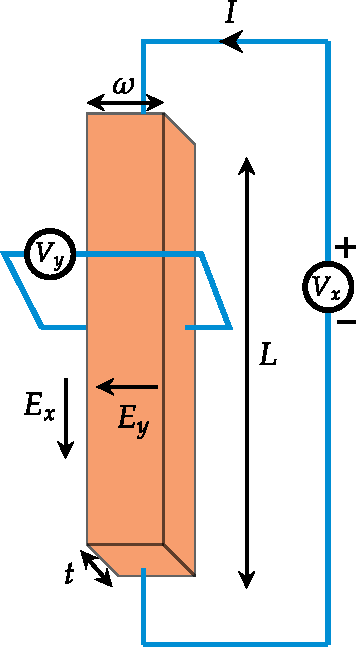
\includegraphics[height=5.5cm,width=3.5cm]{CMP-24}
	\caption{}
	\label{}
\end{figure}
\begin{align*}
\text { magnetic force: } \vec{F}&=q(\vec{v} \times \vec{B})\\
\overrightarrow{F e}&=-e(\vec{V} \times \vec{B})\\
\vec{F}_{h}&=e(\vec{V} \times \vec{B})\qquad \mu=\frac{e \tau}{m^{*}}
\end{align*}
\textbf{Hall effect in semiconductor}
\begin{align*}
R_{H}=\frac{b \mu_{h}^{2}-n \mu_{e}^{2}}{e\left(p \mu_{R}+n \mu_{e}\right)^{2}}
\end{align*}
1.\quad intrinsic semiconductor
\begin{align*}
R_{H}&=\frac{H_{h}=H_{e}}{e n_{i}\left(H_{h}+H_{e}\right)}\\
\Rightarrow \text {-re }\left(\mu_{h}<\mu_{e}\right)
\end{align*}
2.$n$-type semiconductor
\begin{align*}
&n \mathrm{He}_{e} \gg p \mathrm{H}_{R}\\
&R_{n}=-\frac{1}{n e}\\
&\left(n=N_{d}\right)
\end{align*}
3.p-type semiconductor
\begin{align*}
p \mu_{h} &\gg n \mu_{e}\\
R_{H}&=+\frac{1}{p e}\\
&(p=N a)
\end{align*}
\textbf{Hall Effect in Metals}
\begin{align*}
R_{H}&=-\frac{1}{n e}\\
\text { Because metals have only } e^{\theta} s&\text { as charge carriers. }\\
\text { as } E_{F} \alpha n^{2 / 3} &\text { for } 3 \rightarrow\\
n &\propto E_{f}^{3 / 2}\\
\Rightarrow R_{H}& \propto \frac{1}{E_{F}^{3 / 2}}=E_{F}^{-3 / 2}
\end{align*}
\textbf{Hall Coefficient}
\begin{align*}
R_{H}&=\frac{E_{H}}{J_{x} B_{2}}\\
U_{H}&=-\frac{I_{x} B_{2}}{n e t}\\
\text { Hall voltage }&\\
n \rightarrow \operatorname{con} c .&\\
n_{\text {metal }}>&n_{\text {semicon ductor }}\\
R_{\text {metal }}&<R_{H} s\mid c
\end{align*}
\section{Superconductivity}
\subsection{Properties of Superconductors}
\begin{figure}[H]
	\centering
	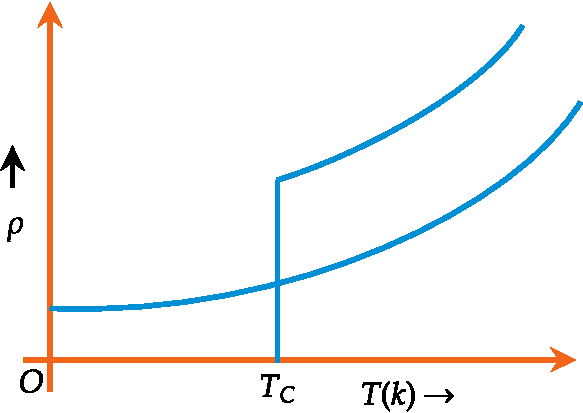
\includegraphics[height=3cm,width=4.5cm]{CMP-5}
	\caption{}
	\label{}
\end{figure}
\begin{enumerate}
	\item At room temperature, the resistivity of $\rho$ of super conducting materials is greater than other element shows as
	\item All thermoelectric effects disappear in super conducting state.
	\item  When a sufficient strong magnetic field is applied to super conductor below critical temperature $\mathrm{T}_{\mathrm{C}}$, it super conducting property is destroyed.
	\item When current is passed through the super conducting materials, the heating loss $\left(I^{2} R\right)$ is zero.
	\begin{align*}
		\text{	As resistivity}\quad \rho&=\frac{R A}{l} \quad \rho \rightarrow \text { very small (zero at } \mathrm{T}_{\mathrm{C}} \text { ) }\\
		\mathrm{R}&=0 \text { Hence no heating loss. }
	\end{align*}
	\item Flux quantization due to ring is $\phi=n \frac{h}{2 e}$
\end{enumerate}
\section{Meissner Effect}
Meissner and ochsenfeld found that if a super conductor is cooled in a magnetic field to below the critical temperature (transition temperature) then at the transition, the lines of induction are pushed out. The expulsion of magnetic flux from the interior of a piece of super-conducting material as the material undergoes the transition to the super-conducting phase is known as Meissner effect. Figure show the normal sphere at $\mathrm{T}>\mathrm{T}_{\mathrm{C}}$ and super conducting sphere at $\mathrm{T}<\mathrm{T}_{\mathrm{C}}$ showing the expulsion of magnetic lines of induction. Meissner effect is reversible when the temperature is raised from below $T_{C}$ the flux suddenly penetrates the specimen after it reaches $T_{C}$ and the substance is in the normal state.
\begin{figure}[H]
	\centering
	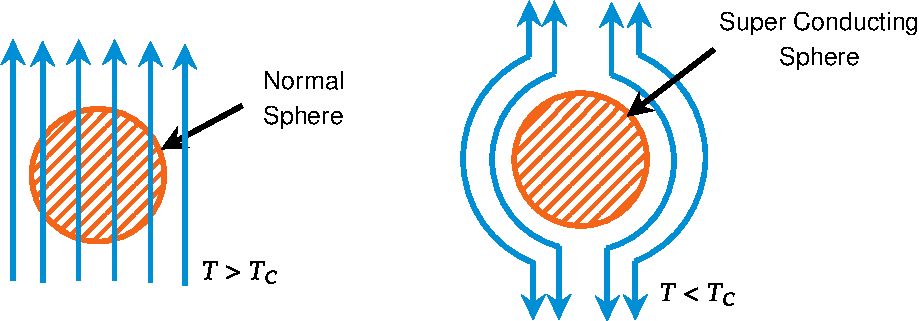
\includegraphics[height=2.8cm,width=8cm]{CMP-6}
	\caption{}
	\label{}
\end{figure}
\begin{align*}
text{As }\quad 
\vec{B}&=\mu_{0}(\vec{H}+\vec{M})\\
\vec{B}&=\mu_{0}(1+x) \vec{H}
\text{where }x=\frac{\vec{M}}{\vec{H}}\\
Since
\vec{B}&=0\text{ for super conductor state}\\
\chi=-1 \text { and also } \chi&=\mu_{\mathrm{r}}-1\quad \text { hence } \mu_{\mathrm{r}}=0
\end{align*}
i.e. a super conductor exhibit perfect diamagnetism. Because of diamagnetic nature, superconducting materials strongly repel external magnet, it leads to a levitation effect.
\subsubsection{Properties of Superconductor}
\subsubsection{Critical Field}
The minimum applied magnetic field necessary to destroy super conductivity and restore the normal resistivity is called the critical field $\mathrm{H}_{\mathrm{C}}$, when the magnetic field exceeds the critical value $\mathrm{H}_{\mathrm{C}}$, the super conducting state is destroyed and the material goes into the normal state. Figure shows the critical field $\mathrm{H}_{\mathrm{C}}$ as a function of temperature. A specimen is superconducting below the curve and normal above the curve. \\
For a given substance, value of $\mathrm{H}_{\mathrm{C}}$ decrease as temperature increases from $\mathrm{T}=0 \mathrm{~K}$ to $\mathrm{T}_{\mathrm{C}}$ (Critical temperature) the curve is nearly parabolic and can be presented as
\begin{figure}[H]
	\centering
	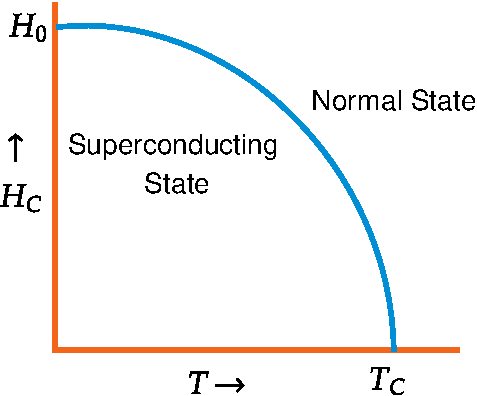
\includegraphics[height=3.3cm,width=4.2cm]{CMP-7}
	\caption{}
	\label{}
\end{figure}
\begin{align*}
H_{C}&=H_{0}\left[1-\left(\frac{T}{T_{C}}\right)^{2}\right]\\
\text { where } \mathrm{H}_{0} &\text { is the critical field at } 0 \mathrm{~K} \text {. }\\
\text { thus the field has its maximum value } &\mathrm{H}_{0} \text { at } \mathrm{T}=0 \mathrm{~K}\\
\text { at } \mathrm{T}=0 \quad H_{C}&=H_{0}\left[1-\frac{0}{T_{C}^{2}}\right]=H_{0}\\
\text { at } \mathrm{T}=\mathrm{T}_{\mathrm{C}} \quad H_{C}&=H_{0}[1-1]=0
\intertext { Equation is the phase boundary between the normal and super conducting state. }
\end{align*}
\begin{exercise}
 The critical field for niobium is $1 \times 10^{5} \mathrm{~A} / \mathrm{m}$ at $8 \mathrm{k}$ and $2 \times 10^{5} \mathrm{~A} / \mathrm{m}$ at $0 \mathrm{~K}$. Calculate the critical temperature of the material.
\end{exercise}
\begin{answer}
	\begin{align*}
	T_{C}=\frac{T}{\left[1-\left(\frac{H_{C}}{H}\right)\right]^{1 / 2}}=11.31 \mathrm{~K}
	\end{align*}
\end{answer}
\subsubsection{Critical Current Density}
The minimum current that can be passed in a sample without destroying its superconductivity is called critical current $\mathrm{I}_{\mathrm{C}}$ and its flux will $\phi=\left(\frac{h}{2 e}\right)$. If a super conducting material carries a current such that the magnetic field which it produce is equal to $\mathrm{H}_{\mathrm{C}}$, the super conductivity disappears. The current density $\mathrm{J}$ at which the super conductivity disappear is called the critical current density $\mathrm{J}_{\mathrm{C}}$ for any value of $\mathrm{J}<\mathrm{J}_{\mathrm{C}}$ the current can sustain itself whereas for values of $\mathrm{J}>$ $\mathrm{J}_{\mathrm{C}}$ the current cannot sustain itself. This effect is known as Silsbee effect.
A super conducting ring of radius $r$ ceases to be a super conductor when the current is
\begin{figure}[H]
	\centering
	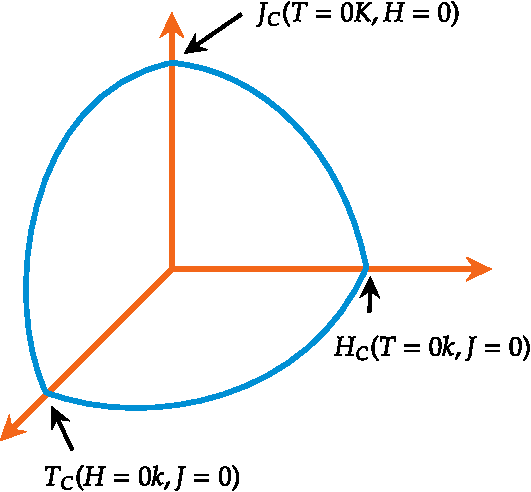
\includegraphics[height=4.5cm,width=5cm]{CMP-8}
	\caption{}
	\label{}
\end{figure}
\begin{align*}
\mathrm{I}_{\mathrm{C}}&=2 \pi \mathrm{rH}_{\mathrm{C}}\\
\text { Critical current density } J_{C}&=\frac{I_{C}}{\text { Area }}=\frac{2 \pi r H_{C}}{\pi r^{2}}\\
J_{C}&=\frac{2 H_{C}}{r}\\
\text { Dependence of } \mathrm{J}, \mathrm{H} \text { and } \mathrm{T} &\text { is shown in figure as }
\end{align*}
\subsubsection{London Penetration Depth}
When a magnetic field is applied to a superconductor, the applied field does not suddenly drop to zero at the surface, instead $\mathrm{H}$ decays exponentially according to the formula.
\begin{align}
H&=H_{0} e^{-x / \lambda}\label{CMP-1}
\intertext{Where $\mathrm{H}_{0}$ is the applied field on the surface at $\mathrm{x}=0, \mathrm{x}$ is the distance from the specimen penetration depth $\lambda$ varies from 300 to about $5000 $\AA.}
\intertext{Penetration depth $\lambda$ is defined as the effective depth to which magnetic field penetrates a super conductor.}
\intertext{The graphical form of equation (\ref{CMP-1}) shown as Penetration depth $\lambda$ depends strongly on temperature and becomes much larger as $T$ approaches $T_{C}$. It is related to temperature as}\notag
\end{align}
\begin{figure}[H]
	\centering
	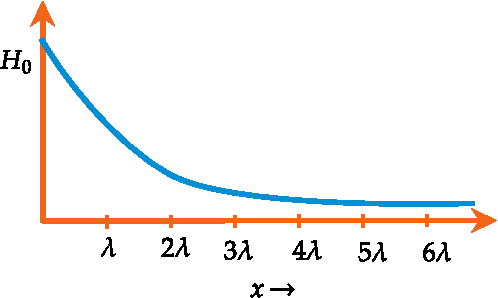
\includegraphics[height=3cm,width=5cm]{CMP-10}
	\caption{}
	\label{}
\end{figure}
\begin{align}
\left[\frac{\lambda(T)}{\lambda(o)}\right]^{2}&=\left[1-\left(\frac{T}{T_{C}}\right)^{4}\right]^{-1}\label{CMP-2}\\
\text{Where }\lambda(\mathrm{T})\text{ and }\lambda(0)&\text{ are the penetration depth at}\notag\\
\mathrm{T} \mathrm{K}\text{ and }0 \mathrm{~K }\text{ respectively.
	}\notag\\
\text{Equation (\ref{CMP-2}) implies that}&\text{ super conducting electron density is given as}\notag\\
n_{s}&=n_{0}\left[1-\left(\frac{T}{T_{C}}\right)^{4}\right]\label{CMP-3}
\intertext{the density of super conducting electron increases from zero to $\mathrm{T}_{\mathrm{C}}$ to $\mathrm{n}_{0}$ at $\mathrm{T}=0 \mathrm{~K}$ as shown in figure}
\end{align}
\begin{figure}[H]
	\centering
	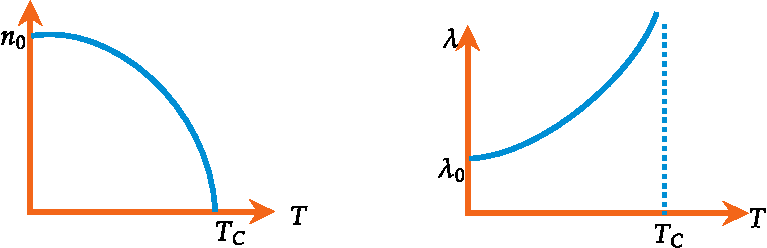
\includegraphics[height=2.8cm,width=8.5cm]{CMP-9}
	\caption{}
	\label{}
\end{figure}
\begin{align}
\text{from equation
	(\ref{CMP-2}) }&\text{and (\ref{CMP-3}) we get}\notag\\
\lambda(T)&=\lambda(0)\left(\frac{n_{0}}{n_{s}}\right)^{1 / 2}\notag\\
\text { Note: London }&\text{equation is defined as }\notag\\
\lambda&=\left(\frac{m}{\mu_{0} n_{s} e^{2}}\right)^{1 / 2} \lambda \propto \sqrt{m}\notag\\
\text { where } &\lambda \text { is London penetration depth. }\notag
\end{align}
\subsubsection{Coherence Length}
The coherence length is measure of the distance within which the gap parameter can not change drastically in a spatially varying magnetic field. It is also a measure of the minimum spatial extent of a transition layer between the normal and super conductor. An intrinsic coherent length $\xi_{0}$ is given as
$$
\xi_{0}=\frac{2 \hbar V_{F}}{\pi E g}
$$
Where $V_{F}$ is electron velocity at the Fermi surface and Eg is energy gap, $\xi_{0}$ is characteristic of pure super conductor. In impure materials and alloys the coherence length is shorter than $\xi_{0}$.
\begin{exercise}
	 Calculate the value of the intrinsic coherence length $\xi_{0}$ for pure mercury whose $\mathrm{T}_{\mathrm{C}}=$ $4.15 \mathrm{~K}$ [Given $\left.\mathrm{V}_{\mathrm{F}}=10^{6} \mathrm{~m} / \mathrm{s}\right]$
\end{exercise}
\begin{answer}
	\begin{align*}
	\xi_{0}&=\frac{2 \hbar V_{F}}{\pi E g}, \mathrm{Eg}=3.53 \mathrm{~K}_{\mathrm{B}} \mathrm{T}_{\mathrm{C}}\\
	\xi_{0}&=331.1 \mathrm{~nm}
	\end{align*}
\end{answer}
\subsubsection{Isotop Effect}
In $1950 \mathrm{C}$ A Reynolds and $\mathrm{E}$. M. Maxwell found that the critical temperature $\mathrm{T}_{\mathrm{C}}$ varies with the atomic mass $\mathrm{M}^{\infty}$ according to the relation
$$\propto=-\frac{\partial \ln T_{C}}{\partial \ln M}=\frac{1}{2} \quad \Rightarrow \quad T_{C} M^{1 / 2}=\text{ constant}$$
Thus, the larger the isotropic mass, lower is transition temperature. For example, the transition temperature of mercury changes from $4.185 \mathrm{~K}$ to $4.146 \mathrm{~K}$. When its isotopic mass is change from $199.5$ to $203.4 \mathrm{amu}$. Now it is known that the mean square amplitude of atomic or lattice vibrations at low temperature is proportional to $\frac{1}{\sqrt{M}}$ and Deye temperature $\mathrm{Q}_{\mathrm{D}}$, of the phonon spectrum is related to $M$ as
\begin{figure}[H]
	\centering
	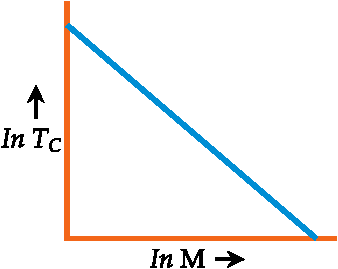
\includegraphics[height=3cm,width=4cm]{CMP-11}
	\caption{}
	\label{}
\end{figure}
\begin{align*}
Q_{D} \sqrt{M}&=\text { constant }\\
\text { From equation (i) and (ii) we get } &\frac{T_{C}}{Q_{D}}=\text { constant }\\
\text { In general, we can write as } &T_{C} \propto Q_{D} \propto \frac{1}{\sqrt{M}}
\end{align*}
\subsubsection{Type-I and Type-II Superconductors}
Superconducting materials can be divided into two types, based on their magnetic response. These two types are designated as type I and II.\\
Type I or the ideal superconductors state are completely diamagnetic, that is when these superconductors are placed in a magnetic field, then all the lines of induction are pushed out from the specimen. These superconductors show Meissner effect. As Magnetic field is increased, the material remains diamagnetic until the critical value $\mathrm{H}_{\mathrm{C}}$ is reached. At this point conduction becomes normal and complete magnetic flux penetration takes place.\\
Type II or hard super conductors are those in which the ideal behavior is seen up to a lower critical field $\mathrm{H}_{\mathrm{C}}$, beyond which the magnetization gradually changes and attains zero at an upper critical field designated as $H_{C_{2}}$. The Meissner effect is incomplete in this region between $H_{C_{1}}$ and $H_{C_{2}}$, this region is known as the Vortex region as shown in figure. The Normal behaviour is observed only beyond $H_{C_{2}}$. The lines of induction penetrate gradually from the specimen as the field is increased beyond $H_{C_{1}}$ and the penetration complete at $H_{C_{2}}$. Figures show the behavior of type I and type II super conductor as a function of $\mathrm{M}$ and $\mathrm{H}$. It is clear that for type I super conductor, upto $\mathrm{H}_{\mathrm{C}}$, the magnetization of the material grows in proportion to the external magnetic field and then abruptly drops to zero at the transition to the normally conducting state.
\begin{figure}[H]
	\centering
	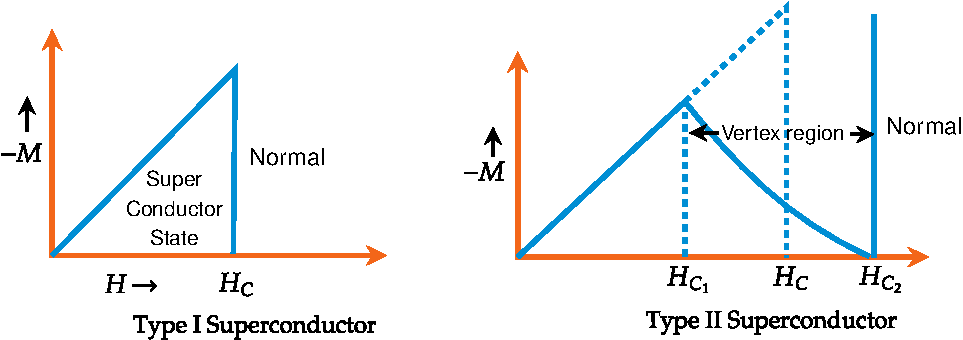
\includegraphics[height=3.8cm,width=10cm]{CMP-12}
	\caption{}
	\label{}
\end{figure}
Variation of resistivity of a type I super conductor and type II super conductor as a function of applied magnetic field is shown in figure.
\begin{figure}[H]
	\centering
	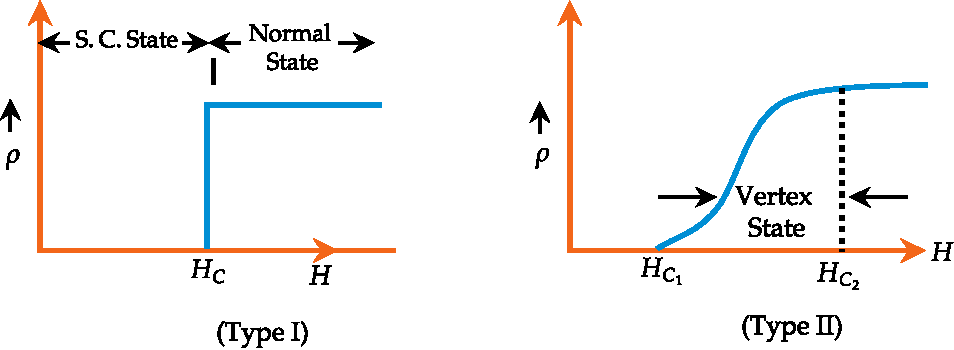
\includegraphics[height=3.4cm,width=8.5cm]{CMP-15}
	\caption{}
	\label{}
\end{figure}
\subsubsection{BCS Theory}
John Bardeen, Lean N. Cooper and John R. Schrieffer developed in 1957 the quantum theory of super conductivity. This theory is based on two experimental results, the isotope effect (as explained earlier) and variation of electronic specific heat with temperature. BCS theory is based on interaction of two electrons through the intermediary of phonons. When an electron approaches an ion in the lattice, there is a coulomb attraction between which causes an increase in the density of ions in the region of distortion. The higher density of ions in the distorted region attracts another electron. Thus a free electron exerts a small attractive force on another electron through phonons with are quanta of lattice vibrations, "A pair of free electrons thus coupled through a phonon is called a cooper pair. Energy of cooper pair is lower than the energy of two individual electrons. The electrons in a cooper pair has opposite spins, so that has a total spin of zero. As a result, the electron pairs in a super conductor are bosons and its radius
\begin{figure}[H]
	\centering
	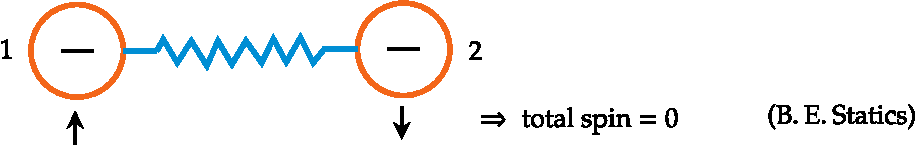
\includegraphics[height=1.5cm,width=9cm]{CMP-13}
	\caption{}
	\label{}
\end{figure}
\begin{align*}
r_{0}&=\left(\frac{\hbar V_{F}}{E_{B}}\right)\\
\Rightarrow \text { total spin }&=0\quad 
\text{(B.E.Statics)}
\intertext{When there are non current in super conductor, the linear momentum of the electrons in a cooper pair are equal and opposite for a total of zero. Energy gap $\mathrm{E}_{\mathrm{g}}$ of a super conductor at $0 \mathrm{~K}$ is given by the formula.}
E_{g}(0)&=3.53 k_{B} T_{C}
\end{align*}
where $\mathrm{k}_{\mathrm{B}}$ is Boltzmann's constant and $\mathrm{T}_{\mathrm{C}}$ is the critical temperature of a super conductor.
At $\mathrm{T}>0 \mathrm{~K}$ some cooper pairs break up. The resulting individual electrons interact with the remaining cooper pair and reduces the energy gap.At critical temperature $\mathrm{TC}$, the energy gap disappears, there are no more cooper pairs, and the material is no longer super conducting. The energy gap Eg can be measured by directly microwave radiation of frequency $\mathrm{v}$ at a super conductor $\mathrm{E}_{\mathrm{g}}$ can also be measured by utilizing the Josephson effect.
\begin{figure}[H]
	\centering
	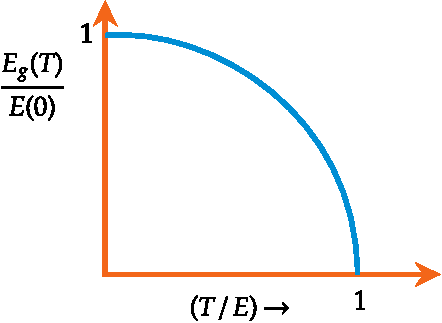
\includegraphics[height=3cm,width=4cm]{CMP-14}
	\caption{}
	\label{}
\end{figure}
\begin{note}
	(i) BCS theory valid only for weak coupling superconductor\\
	(ii) $\mathrm{BCS}$ theory assumed a spherical $\mathrm{FS}$ and isotropic mass.
\end{note}













\newpage
\begin{abox}
	Practise set-1
	\end{abox}
\begin{enumerate}
	\item flux quantum (fluxoid) is approximately equal to $2 \times 10^{-7}$ gauss-cm². A type II superconductor is placed in a small magnetic field, which is then slowly increased till the field starts penetrating the superconductor. The strength of the field at this point is $\frac{2}{\pi} \times 10^{5}$ gauss.\\
	\textbf{A. }The penetrating depth of this superconductor is
{	\exyear{NET/JRF(JUNE-2011)}}
\begin{tasks}(4)
\task[\textbf{A.}] $100 \mathrm{~A}^{0}$ 
\task[\textbf{B.}] $10 \stackrel{0}{\mathrm{~A}}$
\task[\textbf{C.}] $1000 \stackrel{0}{\mathrm{~A}}$
\task[\textbf{D.}] $314 \stackrel{0}{\mathrm{~A}}$
\end{tasks}
\begin{answer}
\begin{align*}
\text{Given Fluxoid }(\phi)_{0}&=2 \times 10^{-7}\text{ gauss }-\mathrm{cm}^{2}\\
\text{First Critical field }\left(H_{c 1}\right)&=\frac{2}{\pi} \times 10^{5}\text{ gauss}
\intertext{The relation between first critical field and penetration depth is}
H_{c 1}&=\frac{\phi_{0}}{\pi \lambda^{2}} \therefore \lambda^{2}=\frac{\phi_{0}}{\pi H_{c 1}}=\frac{2 \times 10^{-7}}{\pi \times \frac{2}{\pi} \times 10^{5}}\\&=10^{-12} \mathrm{~cm}^{2} \Rightarrow \lambda=10^{-6} \mathrm{~cm}=100 \stackrel{0}{\mathrm{~A}}
\end{align*}
So the correct answer is \textbf{Option (A)}
\end{answer}
\textbf{B.} The applied field is further increased till superconductivity is completely destroyed.
The strength of the field is now $\frac{8}{\pi} \times 10^{5}$ gauss. The correlation length of the superconductor is
\begin{tasks}(4)
	\task[\textbf{A.}] $20 \stackrel{0}{\mathrm{~A}}$
	\task[\textbf{B.}] $200 \stackrel{0}{\mathrm{~A}}$
	\task[\textbf{C.}] $628 \stackrel{0}{\mathrm{~A}}$
	\task[\textbf{D.}] $2000 \stackrel{0}{\mathrm{~A}}$
\end{tasks}
\begin{answer}
	\begin{align*}
	\intertext{ Given second critical field $\left(H_{c 2}\right)=\frac{8}{\pi} \times 10^{5}$ gauss. The relation between second critical field and correlation length is $H_{c 2}=\frac{\phi_{0}}{\pi \varepsilon^{2}}$.}
	\therefore \varepsilon^{2}&=\frac{\phi_{0}}{\pi H_{c 2}}=\frac{2 \times 10^{-7}}{\pi \times \frac{8}{\pi} \times 10^{5}}=\frac{1}{4} \times 10^{-12} \mathrm{~cm}^{2} \Rightarrow \varepsilon\\&=\frac{1}{2} \times 10^{-6} \mathrm{~cm}=\frac{100}{2} \times 10^{-10} \mathrm{~m}=50 \text{\AA}
	\end{align*}
	None of the options is matched.
\end{answer}
	\item The potential of a diatomic molecule as a function of the distance $r$ between the atoms is given $\operatorname{by} V(r)=-\frac{a}{r^{6}}+\frac{b}{r^{12}} .$ The value of the potential at equilibrium separation between the atoms is:
	{\exyear{NET/JRF(DEC-2011)}}
\begin{tasks}(4)
\task[\textbf{A.}] $-4 a^{2} / b$
\task[\textbf{B.}] $-2 a^{2} / b$
\task[\textbf{C.}] $-a^{2} / 2 b$
\task[\textbf{D.}] $-a^{2} / 4 b$
\end{tasks}
\begin{answer}
\begin{align*}
\text{Given }V(r)&=-\frac{a}{r^{6}}+\frac{b}{r^{12}} .\\\text{ At equilibrium radius,} \left.\frac{d V(r)}{d r}\right|_{r=r_{0}}&=0\\
\therefore \frac{d V(r)}{d r}&=+\frac{6 a}{r_{0}^{7}}-\frac{12 b}{r_{0}^{13}}=0 \Rightarrow \frac{r_{0}^{13}}{r_{0}^{7}}\\&=\frac{12 b}{6 a}=\frac{2 b}{a} \Rightarrow r_{0}^{6}=\frac{2 b}{a}\\
\therefore\text{ The value of potential at equilibrium is } V\left(r_{0}\right)&=-\frac{a}{r_{0}^{6}}+\frac{b}{r_{0}^{12}}=-\frac{a^{2}}{2 b}+\frac{a^{2}}{4 b}=\frac{-a^{2}}{4 b}
\end{align*}
So the correct answer is \textbf{Option (D)}
\end{answer}
	\item If the number density of a free electron gas in three dimensions is increased eight times, its Fermi temperature will
	{\exyear{NET/JRF(DEC-2011)}}
\begin{tasks}(2)
\task[\textbf{A.}] Increase by a factor of 4
\task[\textbf{B.}]  Decrease by a factor of 4
\task[\textbf{C.}] Increase by a factor of 8
\task[\textbf{D.}]  Decrease by a factor of 8
\end{tasks}
\begin{answer}
\begin{align*}
\intertext{The relation between Fermi energy and electron density is $E_{F}=\frac{\hbar^{2}}{2 m}\left(3 \pi^{2} n\right)^{2 / 3}$.}
\Rightarrow E_{F}^{\prime}&=\frac{\hbar^{2}}{2 m}\left(3 \pi^{2} \times 8 n\right)^{2 / 3}=4 E_{F} \Rightarrow T_{F}^{\prime}=\frac{4 E_{F}}{E_{F}} T_{F}=4 T_{F}
\end{align*}
So the correct answer is \textbf{Option (A)}
\end{answer}
	\item The excitations of a three-dimensional solid are bosonic in nature with their frequency $\omega$ and wave-number $k$ are related by $\omega \propto k^{2}$ in the large wavelength limit. If the chemical potential is zero, the behaviour of the specific heat of the system at low temperature is proportional to
	{\exyear{NET/JRF(DEC-2011)}}
\begin{tasks}(4)
\task[\textbf{A.}]  $T^{1 / 2}$
\task[\textbf{B.}] $T$
\task[\textbf{C.}] $T^{3 / 2}$
\task[\textbf{D.}] $T^{3}$
\end{tasks}
\begin{answer}$\left. \right. $\\
Solution: If the dispersion relation is $\omega \propto k^{s}$ in large wavelength. Then the specific heat is $C_{v} \propto T^{3 / s}$. Given $\omega \propto k^{2} \therefore C_{v} \propto T^{3 / 2}$\\
So the correct answer is \textbf{Option (C)}
\end{answer}
	\item Consider a system of non-interacting particles in $d$ dimensional obeying the dispersion relation $\varepsilon=A k^{s}$, where $\varepsilon$ is the energy, $k$ is the wavevector, $s$ is an integer and $A$ is constant. The density of states, $N(\varepsilon)$, is proportional to
	{\exyear{NET/JRF(JUNE-2012)}}
\begin{tasks}(4)
\task[\textbf{A.}] $\varepsilon^{\frac{s}{d}-1}$
\task[\textbf{B.}] $\varepsilon^{\frac{d}{s}-1}$
\task[\textbf{C.}] $\varepsilon^{\frac{d}{s}+1}$
\task[\textbf{D.}] $\varepsilon^{\frac{s}{d}+1}$
\end{tasks}
\begin{answer}
So the correct answer is \textbf{Option (B)}
\end{answer}
	\item The experimentally measured transmission spectra of metal, insulator and semiconductor thin films are shown in the figure. It can be inferred that I, II and III correspond, respectively, to
	respectively, to
	{\exyear{NET/JRF(JUNE-2012)}}
\begin{figure}[H]
\centering
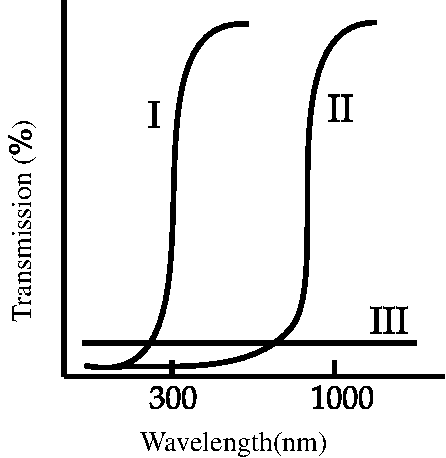
\includegraphics[height=4.5cm,width=4cm]{diagram-20211026(3)-crop}
\end{figure}
\begin{tasks}(2)
\task[\textbf{A.}]  Insulator, semiconductor and metal
\task[\textbf{B.}]  Semiconductor, metal and insulator
\task[\textbf{C.}] Metal, semiconductor and insulator
\task[\textbf{D.}] Insulator, metal and semiconductor
\end{tasks}
\begin{answer}
So the correct answer is \textbf{Option (A)}
\end{answer}
	\item The dispersion relation of phonons in a solid is given by
	$$
	\omega^{2}(k)=\omega_{0}^{2}\left(3-\cos k_{x} a-\cos k_{y} a-\cos k_{z} a\right)
	$$
	The velocity of the phonons at large wavelength is
	{\exyear{NET/JRF(JUNE-2012)}}
\begin{tasks}(4)
\task[\textbf{A.}] $\omega_{0} a / \sqrt{3}$
\task[\textbf{B.}] $\omega_{0} a$
\task[\textbf{C.}] $\sqrt{3} \omega_{0} a$
\task[\textbf{D.}] $\omega_{0} a / \sqrt{2}$
\end{tasks}
\begin{answer}
\begin{align*}
\intertext{For large $\lambda,\left(k_{x} a, k_{y} a, k_{z} a\right)$ are small.}
\omega^{2}(k)&=\omega_{0}^{2}\left[3-\left(1-\frac{k_{x}^{2} a^{2}}{2}\right)-\left(1-\frac{k_{y}^{2} a^{2}}{2}\right)-\left(1-\frac{k_{z}^{2} a^{2}}{2}\right)\right]\\&=\frac{\omega_{0}^{2} a^{2}}{2}\left(k_{x}^{2}+k_{y}^{2}+k_{z}^{2}\right)\\
\omega^{2}(k)&=\frac{\omega_{0}^{2} a^{2}}{2} k^{2} \Rightarrow \omega=\frac{\omega_{0} a}{\sqrt{2}} k \Rightarrow v_{g}=\frac{d \omega}{d k}=\frac{\omega_{0} a}{\sqrt{2}}
\end{align*}
So the correct answer is \textbf{Option (D)}
\end{answer}
	\item A magnetic field sensor based on the Hall Effect is to be fabricated by implanting As into a Si film of thickness $1 \mu \mathrm{m}$. The specifications require a magnetic field sensitivity of $500 \mathrm{mV} /$ Tesla at an excitation current of $1 \mathrm{~mA}$. The implantation dose is to be adjusted such that the average carrier density, after activation, is
	{\exyear{NET/JRF(DEC-2012)}}
\begin{tasks}(2)
\task[\textbf{A.}] $1.25 \times 10^{26} \mathrm{~m}^{-3}$
\task[\textbf{B.}] $1.25 \times 10^{22} \mathrm{~m}^{-3}$
\task[\textbf{C.}] $4.1 \times 10^{21} \mathrm{~m}^{-3}$
\task[\textbf{D.}] $4.1 \times 10^{20} \mathrm{~m}^{-3}$
\end{tasks}
\begin{answer}
\begin{align*}
n&=\frac{I B}{t e V_{H}}=\frac{10^{-3}}{10^{-6} \times 1.6 \times 10^{-19}} \times \frac{1}{500 \times 10^{-3}}\\&=1.25 \times 10^{22} m^{-3}\text{ where }\frac{V_{H}}{B}=500 \times 10^{-3} V / T
\end{align*}
So the correct answer is \textbf{Option (B)}
\end{answer}
	\item In a band structure calculation, the dispersion relation for electrons is found to be
	$$
	\varepsilon_{k}=\beta\left(\cos k_{x} a+\cos k_{y} a+\cos k_{z} a\right)
	$$
	where $\beta$ is a constant and $a$ is the lattice constant. The effective mass at the boundary of the first Brillouin zone is
	{\exyear{NET/JRF(DEC-2012)}}
\begin{tasks}(4)
\task[\textbf{A.}] $\frac{2 \hbar^{2}}{5 \beta a^{2}}$
\task[\textbf{B.}] $\frac{4 \hbar^{2}}{5 \beta a^{2}}$
\task[\textbf{C.}] $\frac{\hbar^{2}}{2 \beta a^{2}}$
\task[\textbf{D.}] $\frac{\hbar^{2}}{3 \beta a^{2}}$
\end{tasks}
\begin{answer}
\begin{align*}
\varepsilon_{k}&=\beta\left(\cos k_{x} a+\cos k_{y} a+\cos k_{z} a\right),\\\text{ Effective mass }m^{*}&=\frac{\hbar^{2}}{\left(\frac{d^{2} \varepsilon_{k}}{d^{2} k}\right)}\\
\text{Brilliouin zone boundary is at }k_{x}&=\pm \frac{\pi}{a}, k_{y}=\pm \frac{\pi}{a}, k_{z}=\pm \frac{\pi}{a}\\
\text{Hence }\left.\left(\frac{d^{2} \varepsilon_{k}}{d^{2} k}\right)\right|_{\frac{\pi}{a}, \underline{\pi}, \frac{\pi}{a}}&=3 \beta a^{2} \Rightarrow m^{*}=\frac{\hbar^{2}}{3 \beta a^{2}}
\end{align*}
So the correct answer is \textbf{Option (D)}
\end{answer}
	\item The radius of the Fermi sphere of free electrons in a monovalent metal with an $\mathrm{fcc}$ structure, in which the volume of the unit cell is $a^{3}$, is
	{\exyear{NET/JRF(DEC-2012)}}
\begin{tasks}(4)
\task[\textbf{A.}] $\left(\frac{12 \pi^{2}}{a^{3}}\right)^{1 / 3}$
\task[\textbf{B.}] $\left(\frac{3 \pi^{2}}{a^{3}}\right)^{1 / 3}$
\task[\textbf{C.}] $\left(\frac{\pi^{2}}{a^{3}}\right)^{1 / 3}$
\task[\textbf{D.}] $\frac{1}{a}$
\end{tasks}
\begin{answer}
\begin{align*}
\text{Radius of Fermi sphere is }k_{F}&=\left(\frac{3 \pi^{2} N}{V}\right)^{1 / 3}, E_{F}=\left(\frac{\hbar^{2}}{2 m}\right)\left(3 \pi^{2} n\right)^{2 / 3}=\left(\frac{\hbar^{2} k_{F}^{2}}{2 m}\right)\\
\text{For fcc solid }\frac{N}{V}&=\frac{4}{a^{3}} \Rightarrow k_{F}=\left(\frac{12 \pi^{2}}{a^{3}}\right)^{1 / 3}
\end{align*}
So the correct answer is \textbf{Option (A)}
\end{answer}
	\item The phonon dispersion for the following one-dimensional diatomic lattice with masses $M_{1}$ and $M_{2}$ (as shown in the figure)\\
	\begin{figure}[H]
		\centering
		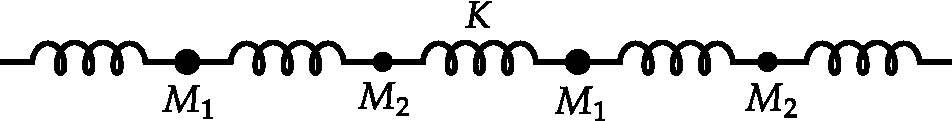
\includegraphics[height=1.3cm,width=9cm]{diagram-20211026(4)-crop}
	\end{figure}
	is given by
	$$
	\omega^{2}(q)=K\left(\frac{1}{M_{1}}+\frac{1}{M_{2}}\right)\left[1 \pm \sqrt{1-\frac{4 M_{1} M_{2}}{\left(M_{1}+M_{2}\right)^{2}} \sin ^{2}\left(\frac{q a}{2}\right)}\right]
	$$
	where $a$ is the lattice parameter and $K$ is the spring constant. The velocity of sound is
	{\exyear{NET/JRF(JUNE-2013)}}
\begin{tasks}(4)
\task[\textbf{A.}] $\sqrt{\frac{K\left(M_{1}+M_{2}\right)}{2 M_{1} M_{2}}} a$
\task[\textbf{B.}] $\sqrt{\frac{K}{2\left(M_{1}+M_{2}\right)} a}$
\task[\textbf{C.}] $\sqrt{\frac{K\left(M_{1}+M_{2}\right)}{M_{1} M_{2}}} a$
\task[\textbf{D.}] $\sqrt{\frac{K M_{1} M_{2}}{2\left(M_{1}+M_{2}\right)^{3}}} a$
\end{tasks}
\begin{answer}
\begin{align*}
\intertext{	For small value of $q$ (i.e. long wavelength approximation limit).}
\text{We have }\sin \left(\frac{q a}{2}\right) \approx \frac{q a}{2}\\
\therefore \omega^{2}(q)&=\mathrm{K}\left(\frac{1}{M_{1}}+\frac{1}{M_{2}}\right)\left[1 \pm \sqrt{1-\frac{4 M_{1} M_{2}}{\left(M_{1}+M_{2}\right)^{2}} \sin ^{2}\left(\frac{q a}{2}\right)}\right]\\
\Rightarrow \omega^{2}(q)&=\mathrm{K}\left(\frac{1}{M_{1}}+\frac{1}{M_{2}}\right)\left[1 \pm \sqrt{1-\frac{4 M_{1} M_{2}}{\left(M_{1}+M_{2}\right)^{2}}\left(\frac{q a}{2}\right)^{2}}\right]\\
\Rightarrow \omega^{2}(q)&=\mathrm{K}\left(\frac{1}{M_{1}}+\frac{1}{M_{2}}\right)\left[1 \pm\left(1-\frac{1}{2} \times \frac{4 M_{1} M_{2}}{\left(M_{1}+M_{2}\right)^{2}} \frac{q^{2} a^{2}}{4}\right)\right]\\
\Rightarrow \omega^{2}(q)&=\mathrm{K}\left(\frac{1}{M_{1}}+\frac{1}{M_{2}}\right)\left[1 \pm\left(1-\frac{M_{1} M_{2}}{\left(M_{1}+M_{2}\right)^{2}} \frac{q^{2} a^{2}}{2}\right)\right]\\
\text{For Acoustical branch:} \omega^{2}(q)&=\mathrm{K}\left(\frac{1}{M_{1}}+\frac{1}{M_{2}}\right)\left[1-\left(1-\frac{M_{1} M_{2}}{\left(M_{1}+M_{2}\right)^{2}} \frac{q^{2} a^{2}}{2}\right)\right]\\
\Rightarrow \omega^{2}(q)&=\mathrm{K}\left(\frac{M_{1}+M_{2}}{M_{1} M_{2}}\right)\left(\frac{M_{1} M_{2}}{\left(M_{1}+M_{2}\right)^{2}} \frac{q^{2} a^{2}}{2}\right)=\frac{\mathrm{K} a^{2}}{2\left(M_{1}+M_{2}\right)} q^{2}\\
\therefore \omega(q)&=\sqrt{\frac{\mathrm{K}}{2\left(M_{1}+M_{2}\right)}} a q\\
\text{Velocity of sound is } v_{g}&=\frac{\omega}{q}=\sqrt{\frac{\mathrm{K}}{2\left(M_{1}+M_{2}\right)}} a
\end{align*}
So the correct answer is \textbf{Option (B)}
\end{answer}
	\item The electron dispersion relation for a one-dimensional metal is given by
	$$
	\varepsilon_{k}=2 \varepsilon_{0}\left[\sin ^{2} \frac{k a}{2}-\frac{1}{6} \sin ^{2} k a\right]
	$$
	where $k$ is the momentum, $a$ is the lattice constant, $\varepsilon_{0}$ is a constant having dimensions of energy and $|k a| \leq \pi .$ If the average number of electrons per atom in the conduction band is $1 / 3$, then the Fermi energy is
	{\exyear{NET/JRF(JUNE-2013)}}
\begin{tasks}(4)
\task[\textbf{A.}] $\varepsilon_{0} / 4$
\task[\textbf{B.}]  $\varepsilon_{0}$
\task[\textbf{C.}] $2 \varepsilon_{0} / 3$
\task[\textbf{D.}] $5 \varepsilon_{0} / 3$
\end{tasks}
\begin{answer}
So the correct answer is \textbf{Option (A)}
\end{answer}
	\item If the energy dispersion of a two-dimensional electron system is $E=u \hbar k$ where $u$ is the velocity and $k$ is the momentum, then the density of states $D(E)$ depends on the energy as
	{\exyear{NET/JRF(JUNE-2013)}}
\begin{tasks}(4)
\task[\textbf{A.}] $1 / \sqrt{E}$
\task[\textbf{B.}] $\sqrt{E}$
\task[\textbf{C.}] $E$
\task[\textbf{D.}] constant
\end{tasks}
\begin{answer}
\begin{align*}
\intertext{In two dimensional system, the number of allowed $k$-states in range $k$ and $k+d k$ is}
g(k) d k&=\left(\frac{L}{2 \pi}\right)^{2} 2 \pi k d k\\
\text{Given dispersion relation is }E&=u \hbar k \therefore k=\frac{E}{u \hbar} \Rightarrow d k=\frac{d E}{u \hbar}\\
\therefore g(E) d E&=\left(\frac{L}{2 \pi}\right)^{2} 2 \pi \times \frac{E}{u \hbar} \times \frac{d E}{u \hbar}=\left(\frac{L}{2 \pi}\right)^{2} \frac{2 \pi}{(u \hbar)^{2}} E d E\\
\Rightarrow \rho(E)&=\frac{g(E) d E}{d E}=\frac{1}{(u \hbar)^{2}} \frac{L^{2}}{2 \pi} E
\end{align*}
So the correct answer is \textbf{Option (C)}
\end{answer}
	\item The energy of an electron in a band as a function of its wave vector $k$ is given by $E(k)=E_{0}-B\left(\cos k_{x} a+\cos k_{y} a+\cos k_{z} a\right)$, where $E_{0}, B$ and $a$ are constants. The effective mass of the electron near the bottom of the band is
	{\exyear{NET/JRF(DEC-2013)}}
\begin{tasks}(4)
\task[\textbf{A.}] $\frac{2 \hbar^{2}}{3 B a^{2}}$
\task[\textbf{B.}] $\frac{\hbar^{2}}{3 B a^{2}}$
\task[\textbf{C.}] $\frac{\hbar^{2}}{2 B a^{2}}$
\task[\textbf{D.}] $\frac{\hbar^{2}}{B a^{2}}$
\end{tasks}
\begin{answer}
\begin{align*}
\intertext{Near the bottom of the band the $k \rightarrow 0$}
\intertext{$\cos k_{x} a \approx 1-\frac{1}{2}\left(k_{x} a\right)^{2}, \cos k_{y} a \approx 1-\frac{1}{2}\left(k_{y} a\right)^{2}, \cos k_{z} a \approx 1-\frac{1}{2}\left(k_{z} a\right)^{2}$}
E(k)&=E_{0}-B\left(\cos k_{x} a+\cos k_{y} a+\cos k_{z} a\right)\\&=E_{0}-B\left(1-\frac{1}{2}\left(k_{x} a\right)^{2}+1-\frac{1}{2}\left(k_{y} a\right)^{2}+1-\frac{1}{2}\left(k_{z} a\right)^{2}\right)\\
&=E_{0}-B\left(3-\frac{1}{2} a^{2}\left(k_{x}+k_{x}+k_{x}\right)^{2}\right)=E_{0}-3 B-\frac{1}{2} B a^{2} k^{2}\\
\text{Effective mass of the electron is }m^{*}&=\frac{\hbar^{2}}{d^{2} E / d k^{2}}=\frac{\hbar^{2}}{B a^{2}}
\end{align*}
So the correct answer is \textbf{Option (D)}
\end{answer}
	\item A uniform linear monoatomic chain is modeled by a spring-mass system of masses $m$ separated by nearest neighbour distance $a$ and spring constant $m \omega_{0}^{2} .$ The dispersion relation for this system is
	{\exyear{NET/JRF(DEC-2013)}}
\begin{tasks}(2)
\task[\textbf{A.}] $\omega(k)=2 \omega_{0}\left(1-\cos \left(\frac{k a}{2}\right)\right)$
\task[\textbf{B.}] $\omega(k)=2 \omega_{0} \sin ^{2}\left(\frac{k a}{2}\right)$
\task[\textbf{C.}] $\omega(k)=2 \omega_{0} \sin \left(\frac{k a}{2}\right)$
\task[\textbf{D.}] $\omega(k)=2 \omega_{0} \tan \left(\frac{k a}{2}\right)$
\end{tasks}
\begin{answer}
\begin{align*}
\intertext{The dispersion relation for uniform linear mono-atomic chain of atoms is}
\omega(k)&=2 \omega_{0} \sin \left(\frac{k a}{2}\right)
\end{align*}
So the correct answer is \textbf{Option (C)}
\end{answer}
	\item The pressure of a nonrelativistic free Fermi gas in three-dimensions depends, at $T=0$, on the density of fermions $n$ as
	{\exyear{NET/JRF(JUNE-2014)}}
\begin{tasks}(4)
\task[\textbf{A.}] $n^{5 / 3}$
\task[\textbf{B.}] $n^{1 / 3}$
\task[\textbf{C.}] $n^{2 / 3}$
\task[\textbf{D.}] $n^{4 / 3}$
\end{tasks}
\begin{answer}
\begin{align*}
\intertext{The Fermi energy in three dimension is defined as}
E_{F}&=\frac{\hbar^{2}}{2 m}\left(\frac{3 \pi^{2} N}{V}\right)^{2 / 3}=\frac{\hbar^{2}}{2 m}\left(3 \pi^{2} n\right)^{2 / 3}
\intertext{Where, n is the electron concentration or density of free Fermi gas.
	The total energy of free Fermi gas in 3D is}
E&=\frac{3}{5} N E_{F}=\frac{3}{5} N \times \frac{\hbar^{2}}{2 m}\left(\frac{3 \pi^{2} N}{V}\right)^{2 / 3}
\intertext{The pressure of a nonrelativistic free Fermi gas is defined as}
p_{F}&=-\left(\frac{\partial E}{\partial V}\right)_{N}=-\frac{3}{5} N \times \frac{\hbar^{2}}{2 m}\left(3 \pi^{2} N\right)^{2 / 3} \times\left(-\frac{2}{3}\right) V^{-5 / 3}\\
&=\frac{2}{5} n E_{F}=\frac{2}{5} n \times \frac{\hbar^{2}}{2 m}\left(3 \pi^{2} n\right)^{2 / 3}=\frac{2}{5} \frac{\hbar^{2}}{2 m}\left(3 \pi^{2}\right)^{2 / 3} n^{5 / 3}
\end{align*}
So the correct answer is \textbf{Option (A)}
\end{answer}
	\item Consider an electron in bec lattice with lattice constant $a$. A single particle wavefunction that satisfies the Bloch theorem will have the form $f(\vec{r}) \exp (\overrightarrow{i k} \cdot \vec{r})$, with $f(\vec{r})$ being
	{\exyear{NET/JRF(JUNE-2014)}}
\begin{tasks}(1)
\task[\textbf{A.}] $1+\cos \left[\frac{2 \pi}{a}(x+y-z)\right]+\cos \left[\frac{2 \pi}{a}(-x+y+z)\right]+\cos \left[\frac{2 \pi}{a}(x-y+z)\right]$
\task[\textbf{B.}] $1+\cos \left[\frac{2 \pi}{a}(x+y)\right]+\cos \left[\frac{2 \pi}{a}(y+z)\right]+\cos \left[\frac{2 \pi}{a}(z+x)\right]$
\task[\textbf{C.}] $1+\cos \left[\frac{\pi}{a}(x+y)\right]+\cos \left[\frac{\pi}{a}(y+z)\right]+\cos \left[\frac{\pi}{a}(z+x)\right]$
\task[\textbf{D.}] $1+\cos \left[\frac{\pi}{a}(x+y-z)\right]+\cos \left[\frac{\pi}{a}(-x+y+z)\right]+\cos \left[\frac{\pi}{a}(x-y+z)\right]$
\end{tasks}
\begin{answer}
\begin{align*}
\intertext{The primitive translational vector for BCC is}
\vec{a}^{\prime}&=\frac{a}{2}(-\hat{i}+\hat{j}+\hat{k}), \vec{b}^{\prime}=\frac{a}{2}(\hat{i}-\hat{j}+\hat{k}), \vec{c}^{\prime}=\frac{a}{2}(\hat{i}+\hat{j}-\hat{k})
\intertext{Bloch function defined as}
\psi_{k}(\vec{r})&=u_{k}(\vec{r}) e^{i \vec{k} \cdot \vec{r}}=f(\vec{r}) e^{i \vec{k} \vec{r}}
\intertext{Here $f(\vec{r})$ is atomic wavefunction, which has the periodicity of the lattice i.e.}
u_{k}(\vec{r}+a)&=u_{k}(\vec{r})
\intertext{Given Bloch function}
f(\vec{r})&=1+\cos \left[\frac{2 \pi}{a}(x+y)\right]+\cos \left[\frac{2 \pi}{a}(y+z)\right]+\cos \left[\frac{2 \pi}{a}(z+x)\right]\\
f\left(\vec{r}+\vec{a}^{\prime}\right)&=1+\cos \left[\frac{2 \pi}{a}\left(x+y-\frac{a}{2}+\frac{a}{2}\right)\right]+\cos \left[\frac{2 \pi}{a}\left(y+z+\frac{a}{2}+\frac{a}{2}\right)\right]+\cos \left[\frac{2 \pi}{a}\left(z+x+\frac{a}{2}-\frac{a}{2}\right)\right]\\
f\left(\vec{r}+\vec{a}^{\prime}\right)&=1+\cos \left[\frac{2 \pi}{a}(x+y)\right]+\cos \left[\frac{2 \pi}{a}(y+z)+2 \pi\right]+\cos \left[\frac{2 \pi}{a}(z+x)\right]\\
f\left(\vec{r}+\vec{a}^{\prime}\right)&=1+\cos \left[\frac{2 \pi}{a}(x+y)\right]+\cos \left[\frac{2 \pi}{a}(y+z)\right]+\cos \left[\frac{2 \pi}{a}(z+x)\right]=f(\vec{r})\\
f\left(\vec{r}+\vec{a}^{\prime}\right)&=f(\vec{r})
\intertext{Similarly,}
f\left(\vec{r}+\vec{b}^{\prime}\right)&=f(\vec{r}) \quad\text{ and } f\left(\vec{r}+\vec{c}^{\prime}\right)=f(\vec{r})
\intertext{Other functions do not satisfy the periodicity}
\end{align*}
So the correct answer is \textbf{Option (B)}
\end{answer}
	\item The dispersion relation for electrons in an f.c.c. crystal is given, in the tight binding approximation, by
	$$
	\varepsilon(k)=-4 \varepsilon_{0}\left[\cos \frac{k_{x} a}{2} \cos \frac{k_{y} a}{2}+\cos \frac{k_{y} a}{2} \cos \frac{k_{z} a}{2}+\cos \frac{k_{z} a}{2} \cos \frac{k_{x} a}{2}\right]
	$$
	where $a$ is the lattice constant and $\varepsilon_{0}$ is a constant with the dimension of energy. The $x$ component of the velocity of the electron at $\left(\frac{\pi}{a}, 0,0\right)$ is
	{\exyear{NET/JRF(JUNE-2014)}}
\begin{tasks}(4)
\task[\textbf{A.}] $-2 \varepsilon_{0} a / \hbar$
\task[\textbf{B.}] $2 \varepsilon_{0} a / \hbar$
\task[\textbf{C.}] $-4 \varepsilon_{0} a / \hbar$
\task[\textbf{D.}] $4 \varepsilon_{0} a / \hbar$
\end{tasks}
\begin{answer}
\begin{align*}
\intertext{Group velocity of electron in dispersive medium is expressed as}
\vec{v}&=\frac{1}{\hbar} \frac{d \varepsilon}{d k}=\frac{1}{\hbar}\left[\frac{d \varepsilon}{d k_{x}} \hat{i}+\frac{d \varepsilon}{d k_{y}} \hat{j}+\frac{d \varepsilon}{d k_{z}} \hat{k}\right]=\vec{v}_{x} \hat{i}+\vec{v}_{y} \hat{j}+\vec{v}_{z} \hat{k}\\
\vec{v}&=\frac{2 \varepsilon_{0} a}{\hbar}\left[\begin{array}{l}\left(\sin \frac{k_{x} a}{2} \cos \frac{k_{y} a}{2}+\cos \frac{k_{z} a}{2} \sin \frac{k_{x} a}{2}\right) \hat{i}+\left(\cos \frac{k_{x} a}{2} \sin \frac{k_{y} a}{2}+\sin \frac{k_{y} a}{2} \cos \frac{k_{z} a}{2}\right) \hat{j}+ \\ \left(\sin \frac{k_{z} a}{2} \cos \frac{k_{y} a}{2}+\cos \frac{k_{x} a}{2} \sin \frac{k_{z} a}{2}\right) \hat{k}\end{array}\right]\\
\text{At }&\left(\frac{\pi}{a}, 0,0\right)\\
\vec{v}&=\frac{2 \varepsilon_{0} a}{\hbar}\left[\left(\sin \frac{\pi}{2} \cos 0+\cos 0 \sin \frac{\pi}{2}\right) \hat{i}+\left(\cos \frac{\pi}{2} \sin 0+\sin 0 \cos 0\right) \hat{j}+\left(\cos 0 \sin 0+\sin 0 \cos \frac{\pi}{2}\right) \hat{k}\right]\\
\vec{v}&=\frac{4 \varepsilon_{0} a}{\hbar}[\hat{i}+0 \hat{j}+0 \hat{k}]=[0 \hat{i}+0 \hat{j}+0 \hat{k}]=\vec{v}_{x} \hat{i}+\vec{v}_{y} \hat{j}+\vec{v}_{z} \hat{k}\\
\vec{v}_{x}&=\frac{4 \varepsilon_{0} a}{\hbar}, \vec{v}_{y}=0, \vec{v}_{z}=0
\intertext{	The $x$ - component of velocity is $v_{x}=\frac{4 \varepsilon_{0} a}{\hbar}$}
\end{align*}
So the correct answer is \textbf{Option (D)}
\end{answer}
	\item Consider two crystalline solids, one of which has a simple cubic structure, and the other has a tetragonal structure. The effective spring constant between atoms in the $c$-direction is half the effective spring constant between atoms in the $a$ and $b$ directions. At low temperatures, the behaviour of the lattice contribution to the specific heat will depend as a function of temperature $T$ as
	{\exyear{NET/JRF(DEC-2014)}}
\begin{tasks}(1)
\task[\textbf{A.}] $T^{2}$ for the tetragonal solid, but as $T^{3}$ for the simple cubic solid
\task[\textbf{B.}]  $T$ for the tetragonal solid, and as $T^{3}$ for the simple cubic solid
\task[\textbf{C.}] $T$ for both solids
\task[\textbf{D.}] $T^{3}$ for both solids
\end{tasks}
\begin{answer}
\begin{align*}
\intertext{Solution: The specific heat of solid in three dimensions is proportional to $T^{3}$ and it is independent of crystal structure.}
\begin{array}{ll}\text { In } & 3 D \quad: \quad C_{V} \propto T^{3} \\ \text { In } & 2 D \quad: \quad C_{V} \propto T^{2} \\ \text { In } & 1 D \quad: \quad C_{V} \propto T\end{array}
\end{align*}
So the correct answer is \textbf{Option (D)}
\end{answer}
	\item A superconducting ring carries a steady current in the presence of a magnetic field $\vec{B}$ normal to the plane of the ring. Identify the INCORRECT statement.
	{\exyear{NET/JRF(DEC-2014)}}
\begin{tasks}(1)
\task[\textbf{A.}] The flux passing through the superconductor is quantized in units of $h c / e$,
\task[\textbf{B.}] The current and the magnetic field in the superconductor are time independent.
\task[\textbf{C.}] The current density $\vec{j}$ and $\vec{B}$ are related by the equation $\vec{\nabla} \times \vec{j}+\Lambda^{2} \vec{B}=0$, where $\Lambda$ is a constant
\task[\textbf{D.}] The superconductor shows an energy gap which is proportional to the transition temperature of the superconductor
\end{tasks}
\begin{answer}
\begin{align*}
\intertext{The flux quantization in superconducting ring is $\phi=n \phi_{o}$}
\text{where }\phi_{o}&=\frac{h c}{2 e}\text{ in CGS units and }\phi_{o}=\frac{h}{2 e}\text{ in MKS units.}
\end{align*}
So the correct answer is \textbf{Option (A)}
\end{answer}
	\item The critical magnetic fields of a superconductor at temperatures $4 K$ and $8 K$ are $11 \mathrm{~mA} / \mathrm{m}$ and $5.5 \mathrm{~mA} / \mathrm{m}$ respectively. The transition temperature is approximately
	{\exyear{NET/JRF(JUNE-2015)}}
\begin{tasks}(4)
\task[\textbf{A.}] $8.4 K$
\task[\textbf{B.}] $10.6 \mathrm{~K}$
\task[\textbf{C.}] $12.9 \mathrm{~K}$
\task[\textbf{D.}] $15.0 \mathrm{~K}$
\end{tasks}
\begin{answer}
\begin{align*}
\intertext{The relation between critical field and critical temperature is}
H_{C}(T)&=H_{0}\left[1-\left(\frac{T}{T_{C}}\right)^{2}\right]\\
\text{Let at }T&=T_{1}, H_{C}\left(T_{1}\right), T=T_{2}, H_{C}(T)=H_{C}\left(T_{2}\right)\\
\text{Thus we get} H_{C}\left(T_{1}\right)&=H_{0}\left[1-\left(\frac{T_{1}}{T_{C}}\right)^{2}\right], H_{C}\left(T_{2}\right)=H_{0}\left[1-\left(\frac{T_{2}}{T_{C}}\right)^{2}\right]\\
\frac{H_{C}\left(T_{1}\right)}{H_{C}\left(T_{2}\right)}&=\frac{1-\left(\frac{T_{1}}{T_{C}}\right)^{2}}{1-\left(\frac{T_{2}}{T_{C}}\right)^{2}} \Rightarrow T_{C}=\sqrt{\frac{\frac{H_{C}\left(T_{1}\right)}{H_{C}\left(T_{2}\right)} T_{2}^{2}-T_{1}^{2}}{\frac{H_{C}\left(T_{1}\right)}{H_{C}\left(T_{2}\right)}-1}} \Rightarrow T_{C}\\&=\sqrt{\frac{2(8)^{2}-(4)^{2}}{2-1}} \approx 10.6
\intertext{where $T_{1}=4 k, T_{2}=8 k, H_{C}\left(T_{1}\right)=11 \mathrm{~mA} / \mathrm{m}$ and $H_{C}\left(T_{2}\right)=5.5 \mathrm{~mA} / \mathrm{m}$}
\end{align*}
So the correct answer is \textbf{Option (B)}
\end{answer}
	\item The low-energy electronic excitations in a two-dimensional sheet of grapheme is given by $E(\vec{k})=\hbar v k$, where $v$ is the velocity of the excitations. The density of states is proportional to
	{\exyear{NET/JRF(JUNE-2015)}}
\begin{tasks}(4)
\task[\textbf{A.}] $E$
\task[\textbf{B.}] $E^{\frac{3}{2}}$
\task[\textbf{C.}] $E^{\frac{1}{2}}$
\task[\textbf{D.}] $E^{2}$
\end{tasks}
\begin{answer}
\begin{align*}
\intertext{The number of $k$ - states in range $k$ and $k+d k$ in two dimension is}
g(k) d k&=\left(\frac{L}{2 \pi}\right)^{2} 2 \pi k d k\\
\therefore E&=\hbar v k \Rightarrow d E=\hbar v d k \Rightarrow g(E) d E\\&=\left(\frac{L}{2 \pi}\right)^{2} 2 \pi \times \frac{E}{\hbar v} \times \frac{d E}{\hbar v}=\left(\frac{L}{2 \pi}\right)^{2} \frac{2 \pi}{(\hbar v)^{2}} E d E
\intertext{The density of state is}
\rho(E)&=\frac{g(E) d E}{d E}=\left(\frac{L}{2 \pi}\right)^{2} \frac{2 \pi}{(\hbar v)^{2}} E \Rightarrow \rho(E) \propto E
\end{align*}
So the correct answer is \textbf{Option (A)}
\end{answer}
	\item The dispersion relation of electrons in a 3 -dimensional lattice in the tight binding approximation is given by,
	$$
	\varepsilon_{k}=\alpha \cos k_{x} a+\beta \cos k_{y} a+\gamma \cos k_{z} a
	$$
	where $a$ is the lattice constant and $\alpha, \beta, \gamma$ are constants with dimension of energy. The effective mass tensor at the corner of the first Brillouin zone $\left(\frac{\pi}{a}, \frac{\pi}{a}, \frac{\pi}{a}\right)$ is
	{\exyear{NET/JRF(DEC-2015)}}
\begin{tasks}(2)
\task[\textbf{A.}] $\frac{\hbar^{2}}{a^{2}}\left(\begin{array}{ccc}-1 / \alpha & 0 & 0 \\ 0 & -1 / \beta & 0 \\ 0 & 0 & 1 / \gamma\end{array}\right)$
\task[\textbf{B.}]  $\frac{\hbar^{2}}{a^{2}}\left(\begin{array}{ccc}-1 / \alpha & 0 & 0 \\ 0 & -1 / \beta & 0 \\ 0 & 0 & -1 / \gamma\end{array}\right)$
\task[\textbf{C.}] $\frac{\hbar^{2}}{a^{2}}\left(\begin{array}{ccc}1 / \alpha & 0 & 0 \\ 0 & 1 / \beta & 0 \\ 0 & 0 & 1 / \gamma\end{array}\right)$
\task[\textbf{D.}] $\frac{\hbar^{2}}{a^{2}}\left(\begin{array}{ccc}1 / \alpha & 0 & 0 \\ 0 & 1 / \beta & 0 \\ 0 & 0 & -1 / \gamma\end{array}\right)$
\end{tasks}
\begin{answer}
\begin{align*}
\intertext{The effective mass as a tensor quantity can be written as}
m_{i j}^{\prime \prime}&=\left[\begin{array}{ccc}m_{x x}^{*} & m_{x y}^{*} & m_{x z}^{*} \\ m_{y x}^{*} & m_{y y}^{*} & m_{y z}^{*} \\ m_{z x}^{*} & m_{z y}^{*} & m_{z z}^{*}\end{array}\right]\text{ where }m_{i j}^{*}=\frac{\hbar^{2}}{\left(\frac{\partial^{2} E}{\partial k_{i} \partial k_{j}}\right)}\\
\text{since }\varepsilon_{k}&=\alpha \cos k_{x} a+\beta \cos k_{y} a+\gamma \cos k_{z} a\\
\therefore m_{x x}^{*}&=\frac{\hbar^{2}}{\left(\frac{\partial^{2} \varepsilon}{\partial k_{x} \partial k_{x}}\right)}=\frac{-\hbar^{2}}{\alpha a^{2} \cos k_{x} a}, \quad m_{y y}^{*}=\frac{\hbar^{2}}{\left(\frac{\partial^{2} \varepsilon}{\partial k_{y}^{2}}\right)}=\frac{-\hbar^{2}}{\beta a^{2} \cos k_{y} a}\\
m_{z z}^{*}&=\frac{\hbar^{2}}{\left(\frac{\partial^{2} \varepsilon}{\partial k_{z}^{2}}\right)}=\frac{-\hbar^{2}}{\gamma a^{2} \cos k_{z} a}, \text{ other terms are zero}\\
\text{Now, at }\left(\frac{\pi}{a}, \frac{\pi}{a}, \frac{\pi}{a}\right) ; m_{x x}&=\frac{\hbar^{2}}{\alpha a^{2}}, m_{y y}^{*}=\frac{\hbar^{2}}{\beta a^{2}}, m_{z z}^{*}\\&=\frac{\hbar^{2}}{\gamma a^{2}} \Rightarrow m_{i j}^{*}=\frac{\hbar^{2}}{a^{2}}\left[\begin{array}{ccc}1 / \alpha & 0 & 0 \\ 0 & 1 / \beta & 0 \\ 0 & 0 & 1 / \gamma\end{array}\right]
\end{align*}
So the correct answer is \textbf{Option (C)}
\end{answer}
	\item A thin metal film of dimension $2 \mathrm{~mm} \times 2 \mathrm{~mm}$ contains $4 \times 10^{12}$ electrons. The magnitude of the Fermi wavevector of the system, in the free electron approximation, is 
	{\exyear{NET/JRF(DEC-2015)}}
\begin{tasks}(2)
\task[\textbf{A.}] $2 \sqrt{\pi} \times 10^{7} \mathrm{~cm}^{-1}$
\task[\textbf{B.}] $\sqrt{2 \pi} \times 10^{7} \mathrm{~cm}^{-1}$
\task[\textbf{C.}] $\sqrt{\pi} \times 10^{7} \mathrm{~cm}^{-1}$
\task[\textbf{D.}] $2 \pi \times 10^{7} \mathrm{~cm}^{-1}$
\end{tasks}
\begin{answer}
\begin{align*}
\intertext{ This is the case of two dimensional metal box. The Fermi wave vector of electron in $2-D$ is}
k_{F}=(2 \pi n)^{\frac{1}{2}}&=\left(2 \pi \frac{N}{L^{2}}\right)^{\frac{1}{2}} ; L^{2}=2 m m \times 2 m m\\&=4 \times 10^{-2} \mathrm{~cm}^{2}\\
\Rightarrow k_{F}&=\sqrt{2 \pi}\left(\frac{4 \times 10^{12}}{4 \times 10^{-2} \mathrm{~cm}^{2}}\right)^{\frac{1}{2}}=\sqrt{2 \pi}\left(10^{14} \mathrm{~cm}^{-2}\right)^{\frac{1}{2}}\\&=\sqrt{2 \pi} \times 10^{7} \mathrm{~cm}^{-1}
\end{align*}
So the correct answer is \textbf{Option (B)}
\end{answer}
	\item For an electron moving through a one-dimensional periodic lattice of periodicity $a$, which of the following corresponds to an energy eigenfunction consistent with Bloch's theorem?
	{\exyear{NET/JRF(DEC-2015)}}
\begin{tasks}(2)
\task[\textbf{A.}] $\psi(x)=A \exp \left(i\left[\frac{\pi x}{a}+\cos \left(\frac{\pi x}{2 a}\right)\right]\right)$
\task[\textbf{B.}] $\psi(x)=A \exp \left(i\left[\frac{\pi x}{a}+\cos \left(\frac{2 \pi x}{a}\right)\right]\right)$
\task[\textbf{C.}] $\psi(x)=A \exp \left(i\left[\frac{2 \pi x}{a}+i \cosh \left(\frac{2 \pi x}{a}\right)\right]\right)$
\task[\textbf{D.}] $\psi(x)=A \exp \left(i\left[\frac{\pi x}{a}+i\left|\frac{\pi x}{2 a}\right|\right]\right)$
\end{tasks}
\begin{answer}
\begin{align*}
\text{According to block theorem, }\psi(x+a)&=\psi(x)\\
\psi(x+a)&=A \exp \left\{i\left[\frac{\pi}{a}(x+a)+\cos \left(\frac{2 \pi}{a}(x+a)\right)\right]\right\}\\&=A \exp \left\{i\left[\left(\frac{\pi x}{a}+\pi\right)+\cos \left(\frac{2 \pi x}{a}+2 \pi\right)\right]\right\}\\
&=A \exp \left[i\left\{\frac{\pi}{a}(x+a)+\cos \frac{2 \pi x}{a}\right\}\right]\\&=A \exp \left[i\left(\frac{\pi x}{a}+\cos \frac{2 \pi x}{a}\right)\right]
\end{align*}
So the correct answer is \textbf{Option (B)}
\end{answer}
	\item The band energy of an electron in a crystal for a particular $k$-direction has the form $\varepsilon(k)=A-B \cos 2 k a$, where $A$ and $B$ are positive constants and $0<k a<\pi$. The electron has a hole-like behaviour over the following range of $k$ :
	{\exyear{NET/JRF(JUNE-2016)}}
\begin{tasks}(2)
\task[\textbf{A.}] $\frac{\pi}{4}<k a<\frac{3 \pi}{4}$
\task[\textbf{B.}] $\frac{\pi}{2}<k a<\pi$
\task[\textbf{C.}] $0<k a<\frac{\pi}{4}$
\task[\textbf{D.}] $\frac{\pi}{2}<k a<\frac{3 \pi}{4}$
\end{tasks}
\begin{answer}
\begin{align*}
\varepsilon(k)&=A-B \cos 2 k a, \frac{d \varepsilon}{d k}=2 B a \sin 2 k a, \frac{d^{2} \varepsilon}{d k^{2}}=4 B a^{2} \cos 2 k a\\
\text{Effective mass }m^{*}&=\frac{\hbar^{2}}{d^{2} \varepsilon / d k^{2}}=\frac{\hbar^{2}}{4 B a^{2} \cos 2 k a}
\intertext{Effective mass of electron $\left(m_{e}^{*}\right)$ and effective mass of holes $\left(m_{h}^{*}\right)$ are opposite in sign i.e.,}
\left(m_{h}^{\prime}=-m_{e}^{*}\right)\\
\text{	Now, in the range }&0<k a<\frac{\pi}{4}, \quad m^{*}\text{ is positive}\\
\text{While in the range }&\frac{\pi}{4}<k a<\frac{3 \pi}{4}, m^{*}\text{ is negative}
\intertext{	Thus, electron has hole like behaviour in the region $\frac{\pi}{4}<k a<\frac{3 \pi}{4}$}
\end{align*}
So the correct answer is \textbf{Option (A)}
\end{answer}
	\item Consider a one-dimensional chain of atoms with lattice constant $a$. The energy of an electron with wave-vector $k$ is $\varepsilon(k)=\mu-\gamma \cos (k a)$, where $\mu$ and $\gamma$ are constants. If an electric field $E$ is applied in the positive $x$-direction, the time dependent velocity of an electron is\\
	(In the following $B$ is the constant)
	{\exyear{NET/JRF(DEC-2016)}}
\begin{tasks}(2)
\task[\textbf{A.}] Proportional to $\cos \left(B-\frac{e E}{\hbar} a t\right)$
\task[\textbf{B.}] Proportional to $E$
\task[\textbf{C.}] Independent of $E$
\task[\textbf{D.}] Proportional to $\sin \left(B-\frac{e E}{\hbar}\right.$ at $)$
\end{tasks}
\begin{answer}
\begin{align*}
\intertext{In the presence of electric field E , we can write}
\vec{F}&=-e \vec{E} \Rightarrow \frac{d \vec{p}}{d t}=-e \vec{E} \Rightarrow \hbar \frac{d k}{d t}=-e E\\
\text{Integration gives, }k(t)&=k(0)-\frac{e E}{\hbar} t\\
\text{The group velocity }v&=\frac{d \omega}{d k}=\frac{1}{\hbar} \frac{\partial \varepsilon(k)}{d k}\\
\text{	Since, }\varepsilon(k)&=\mu-\gamma \cos (k a), \qquad \therefore \quad \frac{\partial \varepsilon(k)}{\partial k}=\gamma a \sin k a\\
\text{Thus, }v&=\frac{\gamma a}{\hbar} \sin (k a)
\intertext{Time dependent velocity of electron is}
v(t)&=\frac{\gamma a}{\hbar} \sin [k(t) a]=\frac{\gamma a}{\hbar} \sin \left[\left(k(0)-\frac{e E}{\hbar} t\right) a\right]\\
&=\frac{\gamma a}{\hbar} \sin \left[k(0) a-\frac{e E}{\hbar} a t\right] \Rightarrow v(t)=\frac{\gamma a}{\hbar} \sin \left[B-\frac{e E}{\hbar} a t\right]
\end{align*}
So the correct answer is \textbf{Option (D)}
\end{answer}
	\item  A thin rectangular conducting plate of length $a$ and width $b$ is placed in the $x y$-plane in two different orientations as shown in the figures below. In both cases a magnetic field $B$ is applied in the $z$-direction and a current flows in the $x$ direction due to the applied voltage $V$.\\
	\begin{figure}[H]
		\centering
		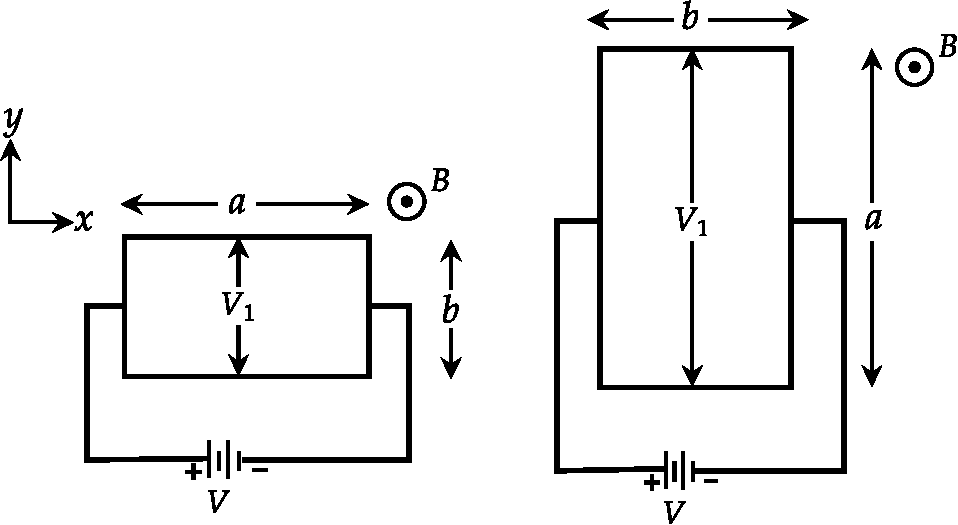
\includegraphics[height=5cm,width=9cm]{diagram-20211026(7)-crop}
	\end{figure}
	If the Hall voltage across the $y$-direction in the two cases satisfy $V_{2}=2 V_{1}$ the ratio $a: b$ must be
	{\exyear{NET/JRF(DEC-2016)}}
\begin{tasks}(4)
\task[\textbf{A.}]  $1: 2$
\task[\textbf{B.}] $1: \sqrt{2}$
\task[\textbf{C.}] $2: 1$
\task[\textbf{D.}] $\sqrt{2}: 1$
\end{tasks}
\begin{answer}
\begin{align*}
\intertext{Since, Hall voltage is given by $V_{H}=\frac{I B}{\rho w}$, where $w$ is width of conducting plate.}
\text{Since, in case (I), }V&=I_{1} R_{1}\text{ and }R_{1}=\frac{\rho l_{1}}{A_{1}}=\frac{\rho a}{a \times b}=\frac{\rho}{b}\\
V&=\frac{I_{1} \rho}{b} \Rightarrow I_{1}=\frac{b V}{\rho}\\
\text{Then, }V_{H}&=V_{1}=\frac{I_{1} B}{\rho w}=\frac{b V B}{\rho^{2} w}=\frac{b V B}{\rho^{2} a}
\qquad(\because w=a)\\
\text{And also in case (II), }R_{2}&=\frac{\rho l_{2}}{A_{2}}=\frac{\rho b}{a \times b}=\frac{\rho}{a}\\
V&=I_{2} R_{2} \Rightarrow I_{2}=\frac{V}{R_{2}}=\frac{V a}{\rho}\\
\text{Then, }V_{H}&=V_{2}=\frac{I_{2} B}{\rho w}=\frac{V a B}{\rho^{2} b}\\
\text{Since, }V_{2}&=2 V_{1} \Rightarrow \frac{a^{2}}{b^{2}}=\frac{2}{1} \Rightarrow a: b=\sqrt{2}: 1
\end{align*}
So the correct answer is \textbf{Option (D)}
\end{answer}
	\item The electrical conductivity of copper is approximately $95 \%$ of the electrical conductivity of silver, while the electron density in silver is approximately $70 \%$ of the electron density in copper. In Drude's model, the approximate ratio $\tau_{C u} / \tau_{A g}$ of the mean collision time in copper $\left(\tau_{C u}\right)$ to the mean collision time in silver $\left(\tau_{A g}\right)$ is
	{\exyear{NET/JRF(JUNE-2017)}}
\begin{tasks}(4)
\task[\textbf{A.}] $0.44$
\task[\textbf{B.}]  $1.50$
\task[\textbf{C.}] $0.33$
\task[\textbf{D.}]  $0.66$
\end{tasks}
\begin{answer}
\begin{align*}
\sigma&=\frac{n e^{2} \tau}{m} \Rightarrow \frac{\sigma_{c u}}{\sigma_{A g}}=\frac{n_{c u}}{n_{A g}} \frac{\tau_{c u}}{\tau_{A g}} \Rightarrow \frac{\tau_{c u}}{\tau_{A g}}=\frac{\sigma_{c u}}{\sigma_{A g}} \times \frac{n_{A g}}{n_{c u}}\\
\Rightarrow \frac{\tau_{c u}}{\tau_{A g}}&=\frac{0.95 \sigma_{A g}}{\sigma_{A g}} \times \frac{0.7 n_{c u}}{n_{c u}} \approx 0.66
\end{align*}
So the correct answer is \textbf{Option (D)}
\end{answer}
	\item The dispersion relation of a gas of spin $\frac{1}{2}$ fermions in two dimensions is $E=\hbar v|\vec{k}|$, where $E$ is the energy, $\vec{k}$ is the wave vector and $v$ is a constant with the dimension of velocity. If the Fermi energy at zero temperature is $\in_{F}$, the number of particles per unit area is
	{\exyear{NET/JRF(DEC-2017)}}
\begin{tasks}(4)
\task[\textbf{A.}] $\frac{\epsilon_{F}}{(4 \pi v \hbar)}$
\task[\textbf{B.}] $\frac{\epsilon_{F}^{3}}{\left(6 \pi^{2} v^{3} \hbar^{3}\right)}$
\task[\textbf{C.}] $\frac{\pi \in_{F}^{3 / 2}}{\left(3 v^{3} \hbar^{3}\right)}$
\task[\textbf{D.}] $\frac{\epsilon_{F}^{2}}{\left(2 \pi v^{2} \hbar^{2}\right)}$
\end{tasks}
\begin{answer}
\begin{align*}
E&=\hbar v|\vec{k}| \Rightarrow k=\frac{E}{\hbar v} \Rightarrow d k=\frac{d E}{\hbar v}\\
g(E) d E&=2\left(\frac{L}{2 \pi}\right)^{2} .2 \pi \cdot \frac{E}{\hbar v} \cdot \frac{d E}{\hbar v}=\left(\frac{L}{2 \pi}\right)^{2} \cdot \frac{4 \pi}{(\hbar v)^{2}} E \cdot d E\\
\text{at }T&=0 K\\
N&=\int_{0}^{E_{F}} g(E) d E=\frac{L^{2}}{4 \pi^{2}} \frac{4 \pi}{(\hbar v)^{2}} \cdot \frac{\epsilon_{F}^{2}}{2}\\
N&=\frac{L^{2}}{2 \pi \hbar^{2} v^{2}} \epsilon_{F}^{2}\\
n&=\frac{N}{L^{2}}=\frac{\epsilon_{F}^{2}}{2 \pi v^{2} \hbar^{2}}
\end{align*}
So the correct answer is \textbf{Option (D)}
\end{answer}
	\item The dispersion relation for the electrons in the conduction band of a semiconductor is given by $E=E_{0}+\alpha k^{2}$ where $\alpha$ and $E_{0}$ are constants. If $\omega_{c}$ is the cyclotron resonance frequency of the conduction band electrons in a magnetic field $B$, the value of $\alpha$ is
	{\exyear{NET/JRF(JUNE-2018)}}
\begin{tasks}(4)
\task[\textbf{A.}] $\frac{\hbar \omega_{c}}{4 e B}$
\task[\textbf{B.}] $\frac{2 \hbar^{2} \omega_{c}}{e B}$
\task[\textbf{C.}] $\frac{\hbar^{2} \omega_{c}}{e B}$
\task[\textbf{D.}]  $\frac{\hbar^{2} \omega_{c}}{2 e B}$
\end{tasks}
\begin{answer}
\begin{align*}
\omega_{c}&=\frac{e B}{m^{*}}\text{ where }m^{*}=\frac{\hbar^{2}}{d^{2} E / d k^{2}}\\
\text{Since }E&=E_{0}+\alpha k^{2} \Rightarrow \frac{d^{2} E}{d k^{2}}=2 \alpha\\
\Rightarrow \omega_{c}&=\frac{e B}{\hbar^{2} / 2 \alpha}=\frac{2 \alpha}{\hbar^{2}} e B \Rightarrow \alpha=\frac{\hbar^{2} \omega_{c}}{2 e B}
\end{align*}
So the correct answer is \textbf{Option (D)}
\end{answer}
\end{enumerate}
 \colorlet{ocre1}{ocre!70!}
\colorlet{ocrel}{ocre!30!}
\setlength\arrayrulewidth{1pt}
\begin{table}[H]
	\centering
	\arrayrulecolor{ocre}
	\begin{tabular}{|p{1.5cm}|p{1.5cm}||p{1.5cm}|p{1.5cm}|}
		\hline
		\multicolumn{4}{|c|}{\textbf{Answer key}}\\\hline\hline
		\rowcolor{ocrel}Q.No.&Answer&Q.No.&Answer\\\hline
		1&\textbf{A} &2&\textbf{D}\\\hline 
		3&\textbf{A} &4&\textbf{C} \\\hline
		5&\textbf{B} &6&\textbf{A} \\\hline
		7&\textbf{D}&8&\textbf{B}\\\hline
		9&\textbf{D}&10&\textbf{A}\\\hline
		11&\textbf{B} &12&\textbf{A}\\\hline
		13&\textbf{C}&14&\textbf{D}\\\hline
		15&\textbf{C}&16&\textbf{A} \\\hline
		17&\textbf{B}&18&\textbf{D}\\\hline
		19&\textbf{D}&20&\textbf{A}\\\hline
		21&\textbf{B} &22&\textbf{A}\\\hline
		23&\textbf{C}&24&\textbf{B}\\\hline
		25&\textbf{B}&26&\textbf{A} \\\hline
		27&\textbf{D}&28&\textbf{D}\\\hline
		29&\textbf{D}&30&\textbf{D}\\\hline
		31&\textbf{D} &&\textbf{}\\\hline
	\end{tabular}
\end{table}
\newpage
\begin{abox}
	Practise set-2
\end{abox}
\begin{enumerate}
	\item The valence electrons do not directly determine the following property of a metal
{	\exyear{GATE 2010}}
\begin{tasks}(2)
\task[\textbf{A.}] Electrical conductivity
\task[\textbf{B.}]  Thermal conductivity
\task[\textbf{C.}] Shear modulus
\task[\textbf{D.}] Metallic luster
\end{tasks}
\begin{answer}
So the correct answer is \textbf{Option (C)}
\end{answer}
	\item The Hall coefficient, $R_{H}$, of sodium depends on
{	\exyear{GATE 2010}}
\begin{tasks}(1)
\task[\textbf{A.}]  The effective charge carrier mass and carrier density
\task[\textbf{B.}] The charge carrier density and relaxation time
\task[\textbf{C.}]  The charge carrier density only
\task[\textbf{D.}] The effective charge carrier mass
\end{tasks}
\begin{answer}
So the correct answer is \textbf{Option (C)}
\end{answer}
	\item  The Bloch theorem states that within a crystal, the wavefunction, $\psi(\vec{r})$, of an electron has the form
{	\exyear{GATE 2010}}
\begin{tasks}(1)
\task[\textbf{A.}]  $\psi(\vec{r})=u(\vec{r}) e^{i \vec{k} \cdot \vec{r}}$ where $\mathrm{u}(\vec{r})$ is an arbitrary function and $\vec{k}$ is an arbitrary vector
\task[\textbf{B.}]  $\psi(\vec{r})=u(\vec{r}) e^{i \vec{G} \cdot \vec{r}}$ where $\mathrm{u}(\vec{r})$ is an arbitrary function and $\vec{G}$ is a reciprocal lattice vector
\task[\textbf{C.}]  $\psi(\vec{r})=u(\vec{r}) e^{i \vec{G} \cdot \vec{r}}$ where $u(\vec{r})=u(\vec{r}+\vec{\Lambda}), \vec{\Lambda}$ is a lattice vector and $\vec{G}$ is a reciprocal lattice vector
\task[\textbf{D.}]  $\psi(\vec{r})=u(\vec{r}) e^{i k, r}$ where $u(\vec{r})=u(\vec{r}+\vec{\Lambda}), \vec{\Lambda}$ is a lattice vector and $\vec{k}$ is an arbitrary vector
\end{tasks}
\begin{answer}
So the correct answer is \textbf{Option (D)}
\end{answer}
	\item In an experiment involving a ferromagnetic medium, the following observations were made. Which one of the plots does NOT correctly represent the property of the medium? ( $T_{C}$ is the Curie temperature)
{	\exyear{GATE 2010}}
\begin{tasks}(2)
\task[\textbf{A.}] \begin{figure}[H]
	\centering
	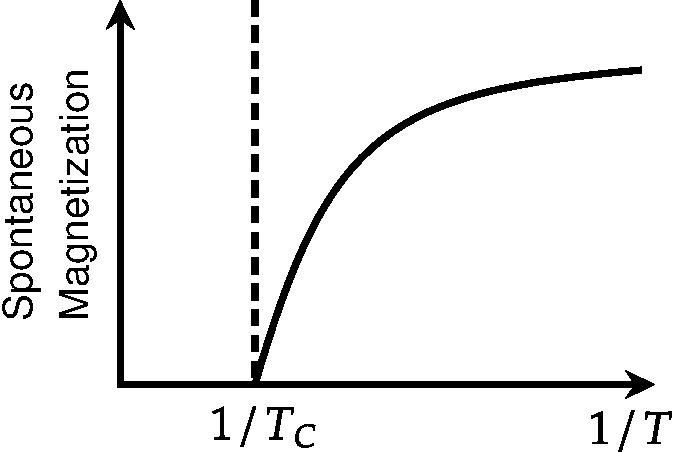
\includegraphics[height=3.5cm,width=4.5cm]{diagram-20210918-crop}
\end{figure}
\task[\textbf{B.}] \begin{figure}[H]
	\centering
	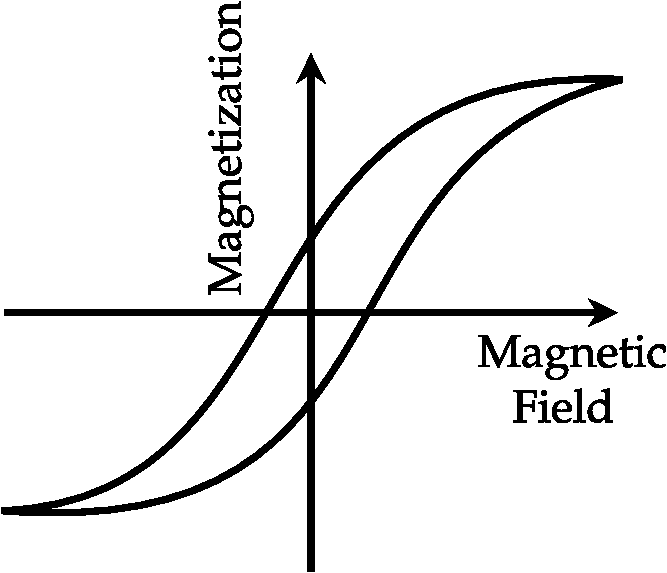
\includegraphics[height=3.5cm,width=4.5cm]{diagram-20210918(1)-crop}
\end{figure}
\task[\textbf{C.}] \begin{figure}[H]
	\centering
	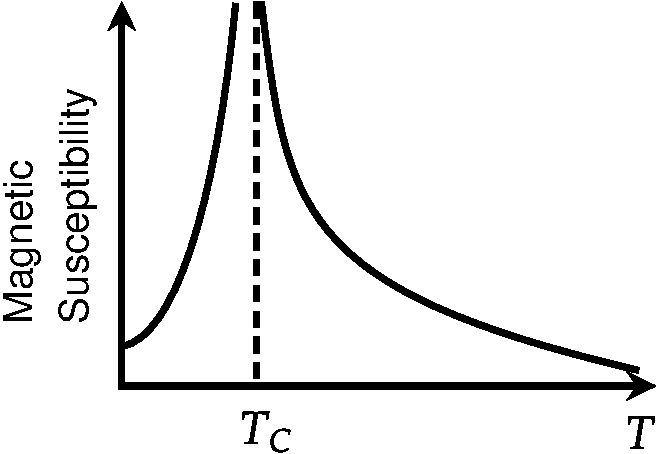
\includegraphics[height=3.5cm,width=4.5cm]{diagram-20210918(2)-crop}
\end{figure}
\task[\textbf{D.}] \begin{figure}[H]
	\centering
	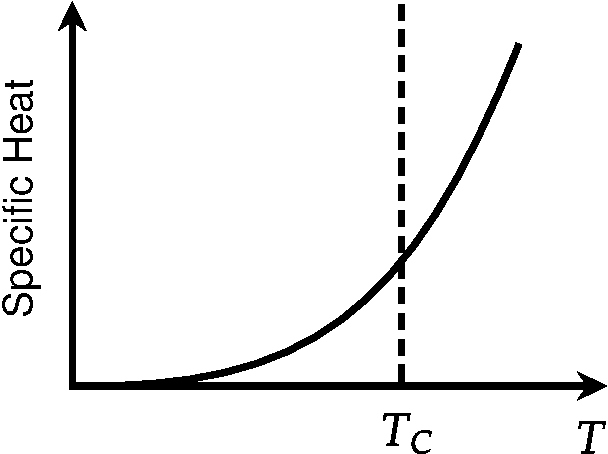
\includegraphics[height=3.5cm,width=4.5cm]{diagram-20210918(3)-crop}
\end{figure}
\end{tasks}
\begin{answer}
So the correct answer is \textbf{Option (C)}
\end{answer}
	\item For a two-dimensional free electron gas, the electronic density $n$, and the Fermi energy $E_{F}$, are related by
{	\exyear{GATE 2010}}
\begin{tasks}(4)
\task[\textbf{A.}] $n=\frac{\left(2 m E_{F}\right)^{3 / 2}}{3 \pi^{2} \hbar^{3}}$
\task[\textbf{B.}] $n=\frac{m E_{F}}{\pi \hbar^{2}}$
\task[\textbf{C.}] $n=\frac{m E_{F}}{2 \pi \hbar^{2}}$
\task[\textbf{D.}] $n=\frac{2^{1 / 3}\left(m E_{F}\right)^{1 / 3}}{\pi \hbar}$
\end{tasks}
\begin{answer}
\begin{align*}
\intertext{For two dimensional gas, the number of possible $k$-states between $k$ and $k+d k$ is}
g(k) d k&=\left(\frac{L}{2 \pi}\right)^{2} 2 \pi k d k=2\left(\frac{L}{2 \pi}\right)^{2} 2 \pi k d k\text{ it is multiplied by 2 for electron gas}\\
\text{	Since }k^{2}&=\frac{2 m E}{\hbar^{2}} \because 2 k d k\\&=\frac{2 m}{\hbar^{2}} d E \Rightarrow 2 \pi k d k=\frac{2 \pi m}{\hbar^{2}} d E\\
\therefore g(E) d E&=2\left(\frac{L}{2 \pi}\right)^{2} \cdot \frac{2 \pi m}{\hbar^{2}} d E
\intertext{The total number of electrons at $T=0^{\circ} \mathrm{K}$ is}
N&=\int_{0}^{E_{F}} g(E) d E \times F(E)=\int_{0}^{E_{F}} g(E) d E\\&=2 \pi \cdot \frac{2 m}{\hbar^{2}}\left(\frac{L}{2 \pi}\right)^{2 E_{F}} d E=2 \pi \cdot \frac{2 m}{\hbar^{2}} \cdot \frac{L^{2}}{4 \pi^{2}} \cdot E_{F}\\
\Rightarrow N&=\frac{m}{\pi \hbar^{2}} \cdot L^{2} E_{F} \Rightarrow E_{F}=\frac{\pi \hbar^{2}}{m}\left(\frac{N}{L^{2}}\right)\\&=\frac{\pi \hbar^{2}}{m} \cdot n \Rightarrow n=\frac{m E_{F}}{\pi \hbar^{2}}
\end{align*}
So the correct answer is \textbf{Option (B)}
\end{answer}
	\item The temperature $(T)$ dependence of magnetic susceptibility $(\chi)$ of a ferromagnetic substance with a Curie temperature $\left(T_{c}\right.$ ) is given by
{	\exyear{GATE 2011}}
\begin{tasks}(1)
\task[\textbf{A.}]  $\frac{C}{T-T_{c}}$, for $T<T_{c}$
\task[\textbf{B.}] $\frac{C}{T-T_{c}}$, for $T>T_{c}$
\task[\textbf{C.}] $\frac{C}{T+T_{c}}$, for $T>T_{c}$
\task[\textbf{D.}] $\frac{C}{T+T_{c}}$, for all temperatures
where $C$ is constant.
\end{tasks}
\begin{answer}
So the correct answer is \textbf{Option (B)}
\end{answer}
	Common Data for Questions 14 and 15:\\
	The tight binding energy dispersion $(E-k)$ relation for electrons in a one-dimensional array of atoms having lattice constant $a$ and total length $L$ is
	$$
	E=E_{0}-\beta-2 \gamma \cos (k a)
	$$
	where $E_{0}, \beta$ and $\gamma$ are constants and $k$ is the wave vector.\\\\
	\item The density of states of electrons (including spin degeneracy) in the band is given by
{	\exyear{GATE 2011}}
\begin{tasks}(4)
\task[\textbf{A.}] $\frac{L}{\pi \gamma a \sin (k a)}$
\task[\textbf{B.}] $\frac{L}{2 \pi \gamma a \sin (k a)}$
\task[\textbf{C.}] $\frac{L}{2 \pi \gamma a \cos (k a)}$
\task[\textbf{D.}] $\frac{L}{\pi \gamma a \cos (k a)}$
\end{tasks}
\begin{answer}
\begin{align*}
D(E)&=2 \times 2\left(\frac{L}{2 \pi}\right) \cdot \frac{1}{d E / d k}\\&=2\left(\frac{L}{2 \pi}\right) \cdot \frac{2 \times 1}{2 a \gamma \sin (k a)}\\&=\frac{2 \times L}{2 \pi \gamma a \sin (k a)}
\end{align*}
So the correct answer is \textbf{Option (A)}
\end{answer}
	\item The effective mass of electrons in the band is given by
{	\exyear{GATE 2011}}
\begin{tasks}(4)
\task[\textbf{A.}] (a) $\frac{\hbar^{2}}{\gamma a^{2} \cos (k a)}$
\task[\textbf{B.}] $\frac{\hbar^{2}}{2 \gamma a^{2} \cos (k a)}$
\task[\textbf{C.}] $\frac{\hbar^{2}}{\gamma a^{2} \sin (k a)}$
\task[\textbf{D.}] $\frac{\hbar^{2}}{2 \gamma a^{2} \sin (k a)}$
\end{tasks}
\begin{answer}
\begin{align*}
\text{	Effective mass }m^{\circ}&=\frac{\hbar^{2}}{\left(\frac{d^{2} E}{d k^{2}}\right)}=\frac{\hbar^{2}}{2 a^{2} \gamma \cos (k a)}\\&=\frac{\hbar^{2}}{2 \gamma a^{2} \cos (k a)}
\end{align*}
So the correct answer is \textbf{Option (B)}
\end{answer}
	\item Which one of the following CANNOT be explained by considering a harmonic approximation for the lattice vibrations in solids?
{	\exyear{GATE 2012}}
\begin{tasks}(2)
\task[\textbf{A.}] Deby's $T^{3}$ law
\task[\textbf{B.}] Dulong Petit's law
\task[\textbf{C.}] Optical branches in lattices
\task[\textbf{D.}]  Thermal expansion
\end{tasks}
\begin{answer}
Solution: Thermal expansion in solid can only be explained if solid behave as a anharmonic oscillator.\\
So the correct answer is \textbf{Option (D)}
\end{answer}
	\item The group velocity at the boundary of the first Brillouin zone is
{	\exyear{GATE 2012}}
\begin{tasks}(4)
\task[\textbf{A.}] 0
\task[\textbf{B.}] 1
\task[\textbf{C.}] $\sqrt{\frac{A a^{2}}{2}}$
\task[\textbf{D.}] $\frac{1}{2} \sqrt{\frac{A a^{2}}{2}}$
\end{tasks}
\begin{answer}
Solution: At the first Brillouin zone the frequency is maximum and the group velocity which is the derivative of the angular frequency is zero.\\\\
So the correct answer is \textbf{Option (A)}
\end{answer}
	\item The energy $\varepsilon_{k}$ for band electrons as a function of the wave vector $k$ in the first Brillouin zone $\left(-\frac{\pi}{a} \leq k \leq \frac{\pi}{a}\right)$ of a one dimensional monoatomic lattice is shown as $(a$ is lattice constant)\\
	\begin{figure}[H]
		\centering
		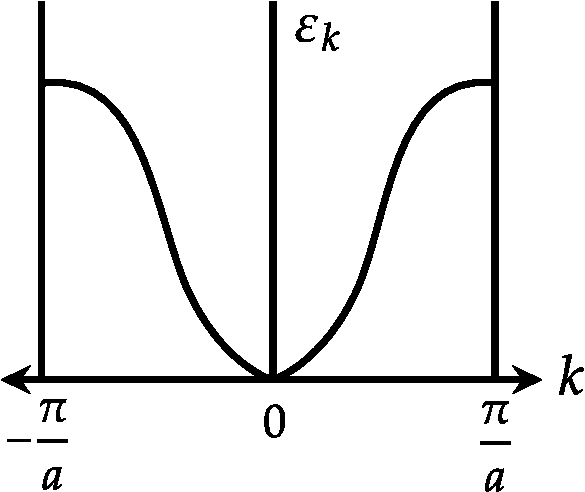
\includegraphics[height=4.5cm,width=5.5cm]{diagram-20210918(10)-crop}
	\end{figure}
	The variation of the group velocity $v_{g}$ is most appropriately represented by
{	\exyear{GATE 2014}}
\begin{tasks}(2)
\task[\textbf{A.}] \begin{figure}[H]
	\centering
	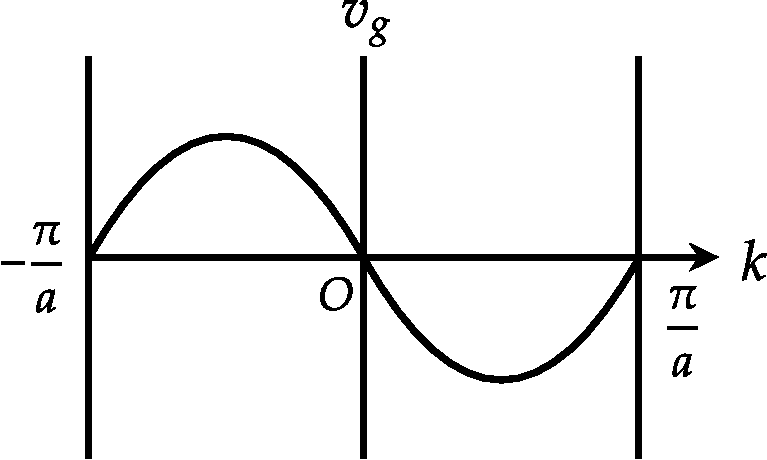
\includegraphics[height=3cm,width=5cm]{diagram-20210918(11)-crop}
\end{figure}
\task[\textbf{B.}] \begin{figure}[H]
	\centering
	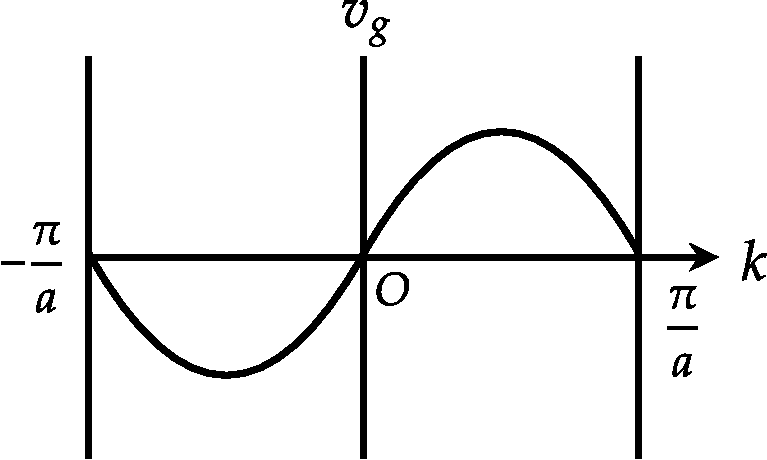
\includegraphics[height=3cm,width=5cm]{diagram-20210918(12)-crop}
\end{figure}
\task[\textbf{C.}] \begin{figure}[H]
	\centering
	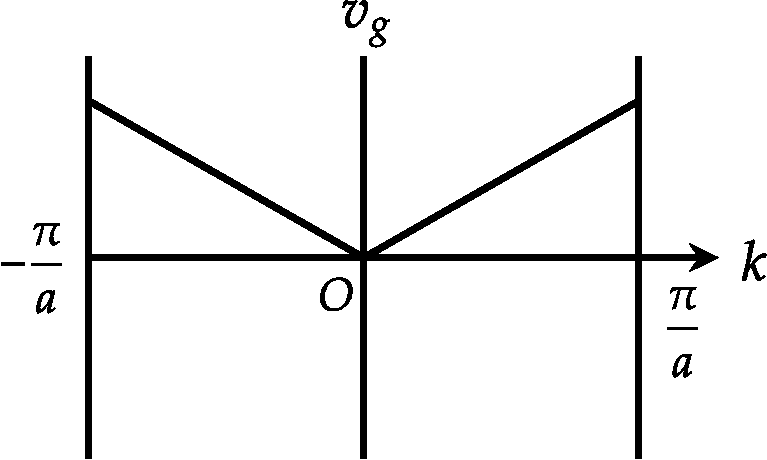
\includegraphics[height=3cm,width=5cm]{diagram-20210918(13)-crop}
\end{figure}
\task[\textbf{D.}] \begin{figure}[H]
	\centering
	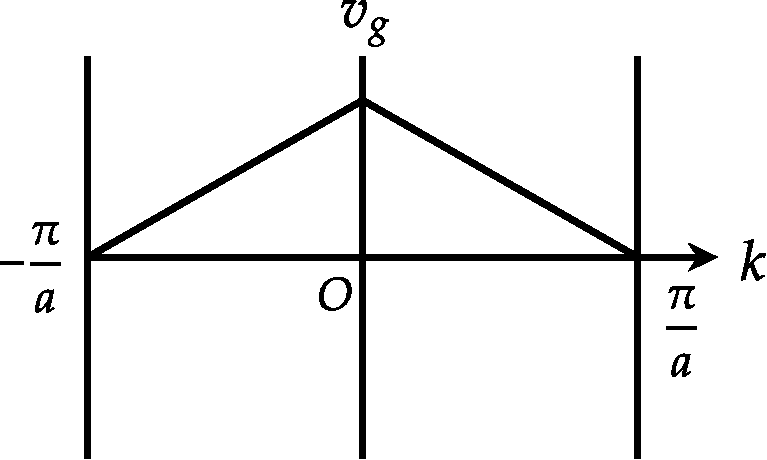
\includegraphics[height=3cm,width=5cm]{diagram-20210918(14)-crop}
\end{figure}
\end{tasks}
\begin{answer}
\begin{align*}
E&=\left(E_{0}-\gamma \beta(\cos k a)\right)\\
V_{g}&=\frac{1}{\hbar} \frac{d E}{d k}=\frac{a \gamma \beta}{\hbar} \sin k a
\end{align*}
So the correct answer is \textbf{Option (B)}
\end{answer}
	\item The energy dependence of the density of states for a two dimensional non-relativistic electron gas is given by, $g(E)=C E^{n}$, where $C$ is constant. The value of $n$ is-----------------
{	\exyear{GATE 2015}}
\begin{answer}
\begin{align*}
\intertext{We know that}
\intertext{$g(E) \propto E^{1 / 2}$ for $3-D, \quad g(E) \propto E^{0}$ for $2-D, g(E) \propto E^{-1 / 2}$ for $1-D$}
\Rightarrow n&=0\text{ for }2-D
\end{align*}
So the correct answer is $0$
\end{answer}
	\item The dispersion relation for phonons in a one dimensional monoatomic Bravais lattice with lattice spacing $a$ and consisting of ions of masses $M$ is given by $\omega(k)=\sqrt{\frac{2 c}{M}[1-\cos (k a)]}$, where $\omega$ is the frequency of oscillation, $k$ is the wavevector and $C$ is the spring constant. For the long wavelength modes $(\lambda>>a)$, the ratio of the phase velocity to the group velocity is---------------
{	\exyear{GATE 2015}}
\begin{answer}
\begin{align*}
\omega(k)&=\sqrt{\frac{2 C}{M}[1-\cos (k a)]}
\intertext{For long wavelength modes $(\lambda>>a)$}
\because \cos (k a) \cong 1-\frac{(k a)^{2}}{2} \Rightarrow \omega(k)&=\sqrt{\frac{2 C}{M}\left[1-1+\frac{(k a)^{2}}{2}\right]}=a \sqrt{\frac{C}{M}} k\\
\text{Phase velocity }v_{P}&=\frac{\omega}{k}=a \sqrt{\frac{C}{M}}\text{ and Group velocity} \\v_{g}&=\frac{d \omega}{d k}=a \sqrt{\frac{C}{M}} \Rightarrow \frac{v_{P}}{v_{g}}=1
\end{align*}
\end{answer}
	\item In a Hall effect experiment, the hall voltage for an intrinsic semiconductor is negative. This is because (symbols carry usual meaning)
	{\exyear{GATE 2015}}
\begin{tasks}(4)
\task[\textbf{A.}] $n \approx p$
\task[\textbf{B.}] $n>p$
\task[\textbf{C.}] $\mu_{n}>\mu_{h}$
\task[\textbf{D.}] $m_{h}^{*}>m_{n}^{*}$
\end{tasks}
\begin{answer}
\begin{align*}
\text{	The Hall voltage is }\quad V_{H}&=R_{H} J B
\intertext{where $J:$ current density, $B:$ magnetic field and $R_{H}:$ Hall constant}
R_{H}&=\frac{1}{e} \frac{p \mu_{p}^{2}-n \mu_{n}^{2}+(p-n) \mu_{n}^{2} \mu_{p}^{2} B^{2}}{\left(n \mu_{n}+p \mu_{p}\right)^{2}+(p-n)^{2} \mu_{n}^{2} \mu_{p}^{2} B^{2}}\\
\text{For intrinsic semiconductor }\left(n=p=n_{i}\right) \quad R_{H}&=\frac{1}{e n_{i}} \frac{\mu_{p}-\mu_{n}}{\mu_{p}+\mu_{n}}
\intertext{In Intrinsic semiconductor $\mu_{n}>\mu_{p}$, therefore Hall voltage is negative.}
\end{align*}
So the correct answer is \textbf{Option (C)}
\end{answer}
	\item Consider a metal which obeys the Sommerfield model exactly. If $E_{F}$ is the Fermi energy of the metal at $T=0 K$ and $R_{H}$ is its Hall coefficient, which of the following statements is correct?
{	\exyear{GATE 2016}}
\begin{tasks}(2)
\task[\textbf{A.}] $R_{H} \propto E_{F}^{\frac{3}{2}}$
\task[\textbf{B.}] $R_{H} \propto E_{F}^{\frac{2}{3}}$
\task[\textbf{C.}] $R_{H} \propto E_{F}^{\frac{-3}{2}}$
\task[\textbf{D.}] $R_{H}$ is independent of $E_{F}$.
\end{tasks}
\begin{answer}
\begin{align*}
R_{H}&=\frac{1}{n e}, \quad\text{ where }E_{F}=\frac{\hbar^{2}}{2 m}\left(3 \pi^{2} n\right)^{2 / 3} \Rightarrow n\\&=\left(\frac{2 m}{\hbar^{2}}\right)^{3 / 2} \cdot \frac{\left(E_{F}\right)^{3 / 2}}{3 \pi^{2}} \Rightarrow R_{H} \propto E_{F}^{-3 / 2}
\end{align*}
So the correct answer is \textbf{Option (C)}
\end{answer}
	\item A one-dimensional linear chain of atoms contains two types of atoms of masses $m_{1}$ and $m_{2}\left(\right.$ where $\left.m_{2}>m_{1}\right)$, arranged alternately. The distance between successive atoms is the same. Assume that the harmonic approximation is valid. At the first Brillouin zone boundary, which of the following statements is correct?
{	\exyear{GATE 2016}}
\begin{tasks}(1)
\task[\textbf{A.}]  The atoms of mass $m_{2}$ are at rest in the optical mode, while they vibrate in the acoustical mode.
\task[\textbf{B.}]  The atoms of mass $m_{1}$ are at rest in the optical mode, while they vibrate in the acoustical mode.
\task[\textbf{C.}] Both types of atoms vibrate with equal amplitudes in the optical as well as in the acoustical modes.
\task[\textbf{D.}] Both types of atoms vibrate, but with unequal, non-zero amplitudes in the optical as well as in the acoustical modes.
\end{tasks}
\begin{answer}
In optical mode, at Brillouin zone boundary atom of heavier mass $\left(m_{2}\right)$ is at rest, whereas in Acoustic mode, atoms of lighter mass $\left(m_{1}\right)$ is at rest.\\
\begin{figure}[H]
	\centering
	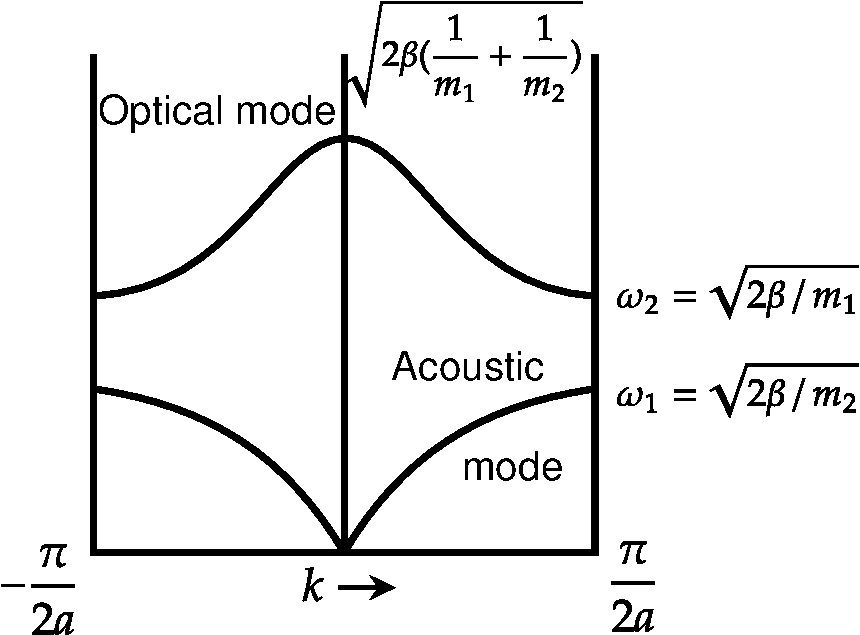
\includegraphics[height=4.5cm,width=6.5cm]{diagram-20210918(19)-crop}
\end{figure}
So the correct answer is \textbf{Option (A)}
\end{answer}
	\item Consider a 2 - dimensional electron gas with a density of $10^{19} \mathrm{~m}^{-2}$. The Fermi energy of the system is................... $e V$ (up to two decimal places).\\
	$\left(m_{e}=9.31 \times 10^{-31} \mathrm{~kg}, h=6.626 \times 10^{-34} \mathrm{Js}, \quad e=1.602 \times 10^{-19} \mathrm{C}\right)$
{	\exyear{GATE 2017}}
\begin{answer}
\begin{align*}
E_{F}&=\left(\frac{\hbar^{2}}{2 m}\right)(2 \pi n)=\frac{\left(1.055 \times 10^{-34} J \cdot s\right)^{2}}{2 \times 9.31 \times 10^{-31}} \times 2 \times 3.142 \times 10^{19}\\
&=0.3756 \times 10^{-18} \mathrm{~J}=0.2345 \times 10 \mathrm{eV}=2.34 \mathrm{eV}
\end{align*}
\end{answer}
	\item At low temperatures $(T)$, the specific heat of common metals is described by (with $\alpha$ and $\beta$ as constants)
{	\exyear{GATE 2018}}
\begin{tasks}(4)
\task[\textbf{A.}] $\alpha T+\beta T^{3}$
\task[\textbf{B.}] $\beta T^{3}$
\task[\textbf{C.}] $\exp (-\alpha / T)$
\task[\textbf{D.}] $\alpha T+\beta T^{5}$
\end{tasks}
\begin{answer}
\begin{align*}
C&=C_{e}+C_{p n}=\alpha T+\beta T^{3}
\end{align*}
So the correct answer is \textbf{Option (A)}
\end{answer}
	\item The energy dispersion for electrons in one dimensional lattice with lattice parameter $a$ is given by $E(k)=E_{0}-\frac{1}{2} W \cos k a$, where $W$ and $E_{0}$ are constants. The effective mass of the electron near the bottom of the band is
{	\exyear{GATE 2018}}
\begin{tasks}(4)
\task[\textbf{A.}] $\frac{2 \hbar^{2}}{W a^{2}}$
\task[\textbf{B.}] $\frac{\hbar^{2}}{W a^{2}}$
\task[\textbf{C.}] $\frac{\hbar^{2}}{2 W a^{2}}$
\task[\textbf{D.}] $\frac{\hbar^{2}}{4 W a^{2}}$
\end{tasks}
\begin{answer}
\begin{align*}
E(k)&=E_{0}-\frac{1}{2} W \cos (k a)\\
\frac{d E}{d k}&=\frac{a W}{2} \sin (k a) \Rightarrow \frac{d^{2} E}{d k^{2}}=\frac{a^{2} W}{2} \cos (k a)\\
\therefore m^{*}&=\frac{\hbar^{2}}{\frac{d^{2} E}{d k^{2}}}=\frac{\hbar^{2}}{\frac{a^{2} W}{2} \cos (k a)}=\frac{2 \hbar^{2}}{W a^{2}}
\intertext{	[At bottom of the band, $k=0$ ]}
\end{align*}
So the correct answer is \textbf{Option (A)}
\end{answer}
	\item In a certain two-dimensional lattice, the energy dispersion of the electrons is
	$$
	\varepsilon(\vec{k})=-2 t\left[\cos k_{x} a+2 \cos \frac{1}{2} k_{x} a \cos \frac{\sqrt{3}}{2} k_{y} a\right]
	$$
	where $\vec{k}=\left(k_{x}, k_{y}\right)$ denotes the wave vector, $a$ is the lattice constant and $t$ is a constant in units of $e V .$ In this lattice the effective mass tensor $m_{i j}$ of electrons calculated at the center of the Brillouin zone has the form $m_{i j}=\frac{\hbar^{2}}{t a^{2}}\left(\begin{array}{cc}\alpha & 0 \\ 0 & \alpha\end{array}\right) .$ The value of $\alpha$ (rounded off to two decimal places) is-----------------
{	\exyear{GATE 2019}}
\begin{answer}
\begin{align*}
\intertext{Effective mass tensor matrix 4}
m_{i j}&=\left[\begin{array}{cc}\frac{1}{m_{x x}} & \frac{1}{m_{x y}} \\ \frac{1}{m_{y x}} & \frac{1}{m_{y y}}\end{array}\right]=\left[\begin{array}{cc}\frac{1}{m_{x x}} & 0 \\ 0 & \frac{1}{m_{y y}}\end{array}\right]\\
\text{	When }m_{x x}&=\frac{\hbar^{2}}{\partial^{2} E / \partial k_{x}^{2}}\text{ and }m_{y y}=\frac{\hbar^{2}}{\partial^{2} E / \partial k_{y}^{2}}\\
\text{Now }\frac{\partial E}{\partial k_{x}}&=2 t\left[a \sin k_{x} a+a \sin \left(\frac{1}{2} k_{x} a\right) \cos \left(\frac{\sqrt{3}}{2} k_{y} a\right)\right]\\
\frac{\partial^{2} E}{d k_{x}^{2}}&=2 t\left[a^{2} \cos \left(k_{x} a\right)+\frac{a^{2}}{2} \cos \left(\frac{1}{2} k_{x} a\right) \cos \left(\frac{\sqrt{3}}{2} k_{y} a\right)\right]\\
\text{At the Brillouin zone centre i.e. at }k_{x}&=k_{y}=0\\
\therefore \quad \frac{\partial^{2} E}{\partial k_{x}^{2}}&=2 t a^{2}\left(1+\frac{1}{2}\right)=3 t a^{2}\\
\text{Similarly, }\frac{\partial E}{\partial k_{y}}&=2 t\left[\sqrt{3} a \cos \left(\frac{1}{2} k_{x} a\right) \sin \left(\frac{\sqrt{3}}{2} k_{y} a\right)\right]\\
\frac{\partial^{2} E}{\partial k_{y}^{2}}&=2 t\left[\frac{3 a^{2}}{2} \cos \left(\frac{1}{2} k_{x} a\right) \cos \left(\frac{\sqrt{3}}{2} k_{y} a\right)\right]\\
\text{At the Brillouin zone centre i.e. at }k_{x}&=k_{y}=0\\
\frac{\partial^{2} E}{\partial_{y}^{2}}&=3 t a^{2}\\
\text{Thus }m_{x x}&=\frac{\hbar^{2}}{\partial^{2} E / \partial k_{x}^{2}}=\frac{\hbar^{2}}{3 t a^{2}}\text{ and }m_{y y}\\&=\frac{\hbar^{2}}{\partial^{2} E / \partial k_{y}^{2}}=\frac{\hbar^{2}}{3 t a^{2}}\\
m_{i j}&=\left[\begin{array}{cc}\frac{\hbar^{2}}{3 t a^{2}} & 0 \\ 0 & \frac{\hbar^{2}}{3 t a^{2}}\end{array}\right]=\frac{\hbar^{2}}{t a^{2}}\left[\begin{array}{cc}\frac{1}{3} & 0 \\ 0 & \frac{1}{3}\end{array}\right]\\
\text{Thus }\alpha&=\frac{1}{3}=0.333
\end{align*}
\end{answer}
\item An ideal gas of non-relativistic fermions in 3-dimensions is at $0 \mathrm{~K}$. When both the number density and mass of the particles are doubled, then the energy per particle is multiplied by a factor
{\exyear{JEST 2014}}
\begin{tasks}(4)
\task[\textbf{A.}]  $2^{1 / 2}$
\task[\textbf{B.}] 1
\task[\textbf{C.}]  $2^{1 / 3}$
\task[\textbf{D.}] $2^{-1 / 3}$
\end{tasks}
\begin{answer}
\begin{align*}
E_{F}&=\frac{\hbar^{2}}{2 m}\left(3 \pi^{2} n\right)^{\frac{2}{3}} \quad\text{ at }T=0 K\\
\because n^{\prime}&=2 n\text{ and }m^{\prime}=2 m \Rightarrow E_{F}^{\prime}=\frac{\hbar^{2}}{4 m}\left(3 \pi^{2} 2 n\right)^{2 / 3}=\frac{\hbar^{2}}{2 m}\left(3 \pi^{2} n\right)^{2 / 3} \times 2^{-1 / 3}
\end{align*}
So the correct answer is \textbf{Option (D)}
\end{answer}
\end{enumerate}
 \colorlet{ocre1}{ocre!70!}
\colorlet{ocrel}{ocre!30!}
\setlength\arrayrulewidth{1pt}
\begin{table}[H]
	\centering
	\arrayrulecolor{ocre}
	\begin{tabular}{|p{1.5cm}|p{1.5cm}||p{1.5cm}|p{1.5cm}|}
		\hline
		\multicolumn{4}{|c|}{\textbf{Answer key}}\\\hline\hline
		\rowcolor{ocrel}Q.No.&Answer&Q.No.&Answer\\\hline
		1&\textbf{C} &2&\textbf{C}\\\hline 
		3&\textbf{D} &4&\textbf{C} \\\hline
		5&\textbf{B} &6&\textbf{B} \\\hline
		7&\textbf{A}&8&\textbf{B}\\\hline
		9&\textbf{D}&10&\textbf{A}\\\hline
		11&\textbf{B} &12&\textbf{0}\\\hline
		13&\textbf{1}&14&\textbf{C}\\\hline
		15&\textbf{C}&16&\textbf{A} \\\hline
		17&\textbf{2.34eV}&18&\textbf{A}\\\hline
		19&\textbf{A}&20&\textbf{0.333}\\\hline
		21&\textbf{D}&&\textbf{}\\\hline
	\end{tabular}
\end{table}

\newpage
\begin{abox}
	Practise set-3
\end{abox}
\begin{enumerate}
	\item 
	The dispersion relation of photons in a solid is:
	$$
	w^{2}(k)=w_{0}^{2}\left[3-\cos k_{x} a-\cos k_{y} a-\cos k_{2} a\right]
	$$
	The velocity of Photons at larger wavelength is:
	\begin{tasks}(2)
		\task[\textbf{a.}] $\frac{\omega_{0} a}{\sqrt{3}}$
		\task[\textbf{b.}]$\omega_{0} a$
		\task[\textbf{c.}]$\sqrt{3} \omega_{0} a$
		\task[\textbf{d.}] $\frac{\omega_{0} a}{\sqrt{2}}$
	\end{tasks}
\begin{answer}
	for larger wavelength (K should be small) 
	\begin{align*}
	\omega^{2}(k)&=\omega_{0}^{2}\left[3-\left(1-\frac{k_{x}^{2} a^{2}}{2}\right)-\left(1-\frac{k_{y}^{2} a^{2}}{2}\right)-\left(1-\frac{k_{2}^{2} a^{2}}{2}\right)\right]\\
	&=\frac{\omega_{0}^{2} a^{2}}{2}\left(k_{x}^{2}+k_{y}^{2}+k_{z}^{2}\right) \\
	&=\frac{\omega_{0}^{2} a^{2}}{2} k^{2} \Rightarrow \omega(k)=\frac{\omega_{0} a}{2} K\\
	V_{g}&=\frac{d \omega}{d k}=\frac{w_{0} a}{\sqrt{2}}
	\end{align*}
	So the correct answer is \textbf{Option (D)}
\end{answer}
\item 
	The phonon dispersion for the following 1-Dim. diatomic lattice with masses $M_{1} \& M_{2}$
	\begin{figure}[H]
		\centering
		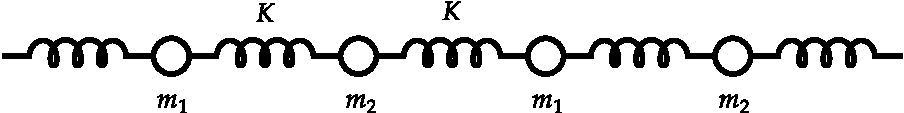
\includegraphics[height=1.2cm,width=9.5cm]{CP-3}
	\end{figure}
	is given by:\\
	$w^{2}(q)=k\left(\frac{1}{m_{1}}+\frac{1}{m_{2}}\right)\left[1 \pm \sqrt{1-\frac{4 M_{1} M_{2}}{\left(M_{1}+M_{2}\right)^{2}} \sin ^{2}\left(\frac{q a}{2}\right)}\right.$\\
	where $a$ is the lattice parameter and $K$ is the spring constant. The velocity of sound is:
\begin{tasks}(2)
	\task[\textbf{a.}]$\sqrt{\frac{K\left(M_{1}+M_{2}\right)}{2 M_{1} M_{2}} a}$
	\task[\textbf{b.}]$\sqrt{\frac{K}{2\left(M_{1}+M_{2}\right)}} a$
	\task[\textbf{c.}]$\sqrt{\frac{K\left(M_{1}+M_{2}\right)}{M_{1} M_{2}}} a$
	\task[\textbf{d.}] done
\end{tasks}
\begin{answer}
	For long wavelength
	\begin{align*}
	\sin ^{2}\left(\frac{q a}{2}\right) &\approx \frac{q^{2} a^{2}}{4}\\
	\omega^{2}&=K\left(\frac{1}{M_{1}}+\frac{1}{M_{2}}\right)\left[1-\sqrt{1-\frac{4 M_{1} M_{2}}{\left(M_{1}+M_{2}\right)^{2}} \cdot \frac{q^{2} a^{2}}{4}}\ \right]\\
	&=K\left(\frac{1}{M_{1}}+\frac{1}{M_{2}}\right)\left[1-\left(1-\frac{1}{2} \cdot \frac{4 M_{1} M_{2}}{\left(M_{1}+M_{2}\right)^{2}} \cdot \frac{q^{2} a^{2}}{4}\right)\right]\\
	&=k\left(\frac{1}{m_{1}}+\frac{1}{m_{2}}\right)\left[\frac{1}{2} \frac{q^{2} a^{2}}{M_{1} M_{2}\left(\frac{1}{M_{1}}+\frac{1}{m_{2}}\right)^{2}}\right]\\
	\omega_{-}^{2}&=\frac{1}{2} k \frac{q^{2} a^{2}}{\left(M_{1}+M_{2}\right)}\\
	v_{\text {sound }}&=\frac{\omega-1 q}{q}=\sqrt{\frac{K}{2\left(M_{1}+M_{2}\right)}} a
	\end{align*}
	So the correct answer is \textbf{Option (B)}
\end{answer}
\item A uniform linear monoatomic chain is modeled by a spring mass system of masses $m$ seperated by nearest neighbour distance $a$ and spring constant $\omega_{0}^{2}$. The dispersion relation for this system is:
	\begin{tasks}(2)
		\task[\textbf{a.}]$\omega(k)=2 \omega_{0}\left[1-\cos \frac{k q}{Q}\right]$
		\task[\textbf{b.}]$\omega(k)=2 \omega \sin ^{2}\left(\frac{k a}{a}\right)$
		\task[\textbf{c.}]$\omega(K)=2 \omega_{0} \sin \left(\frac{k a}{2}\right)$
		\task[\textbf{d.}] $\omega(k)=2 \omega_{0} \tan \left(\frac{k a}{2}\right)$
	\end{tasks}
\begin{answer}
	\begin{align*}
	\omega(k)&=\sqrt{\frac{4 c}{m}} \sin \left(\frac{k a}{2}\right)\quad c=m \omega_{0}^{2}\text{ (given)}\\
	&=\sqrt{\frac{4 cm\omega^{2}_0}{m}} \sin \left(\frac{k g}{2}\right)=2 \omega_{0} \sin \frac{k q}{2}
	\end{align*}
	So the correct answer is \textbf{Option (C)}
\end{answer}
\item A sample of $Si$ has electron and hole mobility of $0.13 \& 0.05 \mathrm{~m}^{2} / \mathrm{vrs}$ respectively at $300 $K.  It is doped with $\rho$ and $Al$ with doping densities of $1.5 \times 20^{21} 1 \mathrm{~m}^{3}$ and $2.5 \times 10^{21} \mathrm{~m}^{3}$ respectively. The conductivity of the doped $Si$ sample at $300$k.
	\begin{tasks}(2)
		\task[\textbf{a.}]$8 n^{-1} m^{-1}$
		\task[\textbf{b.}]$32 \Omega^{-1} \mathrm{~m}^{-1}$
		\task[\textbf{c.}]$20.8\Omega^{-1}m^{-1}$
		\task[\textbf{d.}]  $83.2 \Omega^{-1}m^{-1}$
	\end{tasks}
\begin{answer}
	\begin{align*}
	\text{doping of }Al&>\text{ doping of }\rho\\
	ie \quad\rho-&\text{type semiconductor.}\\
	\text{majority carrier conc }&=(2.5-1.5)\times10^{21}/m^3\\
	&=10^{21}/m^3\\
	\sigma &=p e \mu_{h} \\
	& \approx 10^{21} \times 1.6 \times 10^{-19} \times 0.05\\
	&=8\Omega^{-1}m^{-1}
	\end{align*}
	So the correct answer is \textbf{Option (a)}
\end{answer}
\item 
	The concentration of electrons $n$ and holes $p$ for an intrinsic semiconductor at temperature $T$ can be explained as 
	$$n=p=A T^{3 / 2} \exp \left(-E_{g} \mid 2 K_{B} T\right)$$
	where $Eg$ is the band gap and $A$ is a constant.\\
	If the mobility of both types of carries is proportional to $T^{}3/2$, then the log of the conductivity is a linear function of $T^{-1}$ with slope.
	\begin{tasks}(2)
		\task[\textbf{a.}]$\frac{E g}{2 k_{B}}$
		\task[\textbf{b.}]$\frac{E g}{k_{B}}$
		\task[\textbf{c.}]$-\frac{E g}{2 k_{B}}$
		\task[\textbf{d.}] $\frac{-E g}{K B}$
	\end{tasks}
\begin{answer}$\left. \right. $
	\begin{figure}[H]
		\centering
		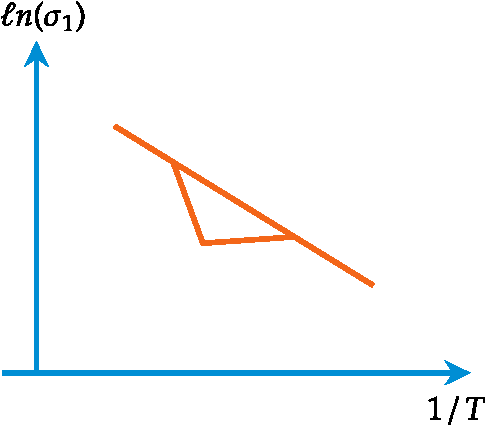
\includegraphics[height=3cm,width=3.5cm]{CMP-23}
		\caption{}
		\label{}
	\end{figure}
	\begin{align*}
	\sigma_{i}&=c T^{3 / 2} \exp \left(\frac{-E g}{2 k_{B} T}\right) \cdot e D T^{-3 / 2}\\
	\therefore \quad \sigma_{i}&=n_{i} e\left(\mu_{e}+\mu_{h}\right)\hspace{1cm}\text { due to }\left(H_{e}+H_{R}\right)\\
	\sigma_{i}&=c \exp \left(\frac{-E g}{2 k_{B} t}\right)\\
	\ln \sigma_{i}&=\ln c-\frac{E g}{2 k_{B} T}\\
	\text { Slope }&=-\frac{E g}{2 t_{B}}
	\end{align*}
	So the correct answer is \textbf{Option (c)}
\end{answer}
\item 
	A junction is made between a metal of work function $\omega_m ,$  and a doped semiconductor of work function $\omega_s$ with $\omega_{M}>\omega_{S} $. If the electronic field at the interface has been increased by a factor of $3$. Then the dopant conc. in S/c would be. 
	\begin{tasks}(2)
		\task[\textbf{a.}]Increase by a
		\task[\textbf{b.}]Decrease by 3
		\task[\textbf{c.}]Increase by 3
		\task[\textbf{d.}]Decrease by $\sqrt{3}$
	\end{tasks}
\begin{answer}
	\begin{align*}
	\vec{E} \text { at metal }-s/c &\text { interface } \alpha\left(N_{d}\right)^{2}\\
	\vec{E} \text { qed by } &=(3)^{2} \\
	&=9 \text { times }
	\end{align*}
	So the correct answer is \textbf{Option (a)}
\end{answer}
\item 
	A magnetic field sensor based on the hall effect is to be facricated by implanting as into a $si$ film of thickness $1\mu m$
	The specifications require a magnetic field ssensitivity of $500 mV/T$ at an excitation current of $1 mA$. The implantation does to be adjusted such that the average carrier density, after acivation is,
	\begin{tasks}(2)
		\task[\textbf{a.}] $1.25 \times 10^{26} \mathrm{~cm}^{-3}$
		\task[\textbf{b.}]$1.25 \times 10^{22} \mathrm{~cm}^{-3}$
		\task[\textbf{c.}]$4.1 \times 10^{21} \mathrm{~cm}^{-3}$
		\task[\textbf{d.}] $4.1 \times 10^{23} \mathrm{~cm}^{-3}$
	\end{tasks}
\begin{answer}
	\begin{align*}\text { magnetic field sensilivity: } \frac{V_{H}}{B}&=500 \times 10^{-3} \frac{\mathrm{V}}{\mathrm{T}}\\
	\operatorname{curent}(I)&=\operatorname{lm} A=10^{-3} \mathrm{~A}\\
	\text { thickness }(t)&=1 \times 10^{-6} \mathrm{~m}\\
	U_{H}&=\frac{I_{x} B_{2}}{n e t} \Rightarrow n=\frac{I_{x} B_{2}}{V_{H} e t}\\
	n&=\frac{10^{-3} \times 1 \mathrm{~T}}{500 \times 10^{-3} \times 1.6 \times 10^{-19}} \times 10^{-6} \\
	n&=1.25 \times 10^{22} \mathrm{~m}^{-3}
	\end{align*}
	So the correct answer is \textbf{Option (b)}
\end{answer}
\end{enumerate}